% !TeX spellcheck = en_GB
% !TeX program = lualatex

\documentclass[a4paper,
               %boxit,        % check whether paper is inside correct margins
               %titlepage,    % separate title page
               %refpage       % separate references
               %biblatex,     % biblatex is used
               keeplastbox,   % flushend option: not to un-indent last line in References
               %nospread,     % flushend option: do not fill with whitespace to balance columns
               %hyphens,      % allow \url to hyphenate at "-" (hyphens)
               %xetex,        % use XeLaTeX to process the file
               %luatex,       % use LuaLaTeX to process the file
               ]{jacow}
%
% ONLY FOR \footnote in table/tabular
%
\usepackage{pdfpages,multirow,ragged2e} %
%
% CHANGE SEQUENCE OF GRAPHICS EXTENSION TO BE EMBEDDED
% ----------------------------------------------------
% test for XeTeX where the sequence is by default eps-> pdf, jpg, png, pdf, ...
%    and the JACoW template provides JACpic2v3.eps and JACpic2v3.jpg which
%    might generates errors, therefore PNG and JPG first
%
\makeatletter%
	\ifboolexpr{bool{xetex}}
	 {\renewcommand{\Gin@extensions}{.pdf,%
	                    .png,.jpg,.bmp,.pict,.tif,.psd,.mac,.sga,.tga,.gif,%
	                    .eps,.ps,%
	                    }}{}
\makeatother

% CHECK FOR XeTeX/LuaTeX BEFORE DEFINING AN INPUT ENCODING
% --------------------------------------------------------
%   utf8  is default for XeTeX/LuaTeX
%   utf8  in LaTeX only realises a small portion of codes
%
\ifboolexpr{bool{xetex} or bool{luatex}} % test for XeTeX/LuaTeX
 {}                                      % input encoding is utf8 by default
 {\usepackage[utf8]{inputenc}}           % switch to utf8

\usepackage[USenglish]{babel}

%
% if BibLaTeX is used
%
\ifboolexpr{bool{jacowbiblatex}}%
 {%
  \addbibresource{jacow-test.bib}
  \addbibresource{biblatex-examples.bib}
 }{}
\listfiles

\usepackage{pgf}

\graphicspath{
    {pictures/photos},
    {pictures/ipe}}
    
\newcommand{\mathdefault}[1][]{}

%%   Lengths for the spaces in the title
%%   \setlength\titleblockstartskip{..}  %before title, default 3pt
%%   \setlength\titleblockmiddleskip{..} %between title + author, default 1em
%%   \setlength\titleblockendskip{..}    %afterauthor, default 1em


\begin{document}

\title{LHC abort gap monitor electronics upgrade}

\author{P. Pacner\thanks{petr.pacner@cern.ch}, Brno University of Technology, Brno, Czech Republic \\
		S. B. Pedersen, D. B\v{e}lohrad, M. Martin Nieto, S. Mazzoni, CERN, Geneva, Switzerland}
	
\maketitle

\begin{abstract}
    The LHC Abort Gap Monitor (AGM) is part of the LHC machine protection
    system (MPS) and is designed to measure the particle population in a 3us
    wide region known as the "abort gap." This region needs to be kept empty to
    ensure safe beam dumps. The AGM captures the synchrotron light generated in
    the visible part of the spectra and converts it into an electric signal.
    This signal is then processed by an acquisition system and can trigger the
    ‘abort gap cleaning’ process. The current AGM, which has been in operation
    since 2010, uses an analogue integrator ASIC and a 40 MHz
    analogue-to-digital (ADC) converter to provide the particle population
    information. However, this solution is now considered obsolete and is being
    replaced by a digital signal processing approach. Working directly in the
    digital domain not only offers more scalability but also better determinism
    and reliability. This work presents the new technical solution for the
    acquisition chain, compares the characteristics of both implementations,
    and showcases recent measurements conducted on the LHC ion and proton
    beams.
\end{abstract}

\section{Introduction}
During the flat-top phase, the LHC ring stores up to \SI{350}{MJ} of beam energy,
spread across 2808 bunches with an average beam transverse size under
\SI{1}{mm}. This high energy density can melt metallic surfaces and quench
superconducting magnets, posing a risk to the machine~\cite{LHC_report}. 
To safely extract the beam from the vacuum compartments, a series of kicker
magnets belonging to the beam dump system is used. These magnets take 3 us to
ramp up their magnetic field~\cite{beam_dump_system}. This defines the size of
an abort gap (AG) in the bunch train. Due to system imperfections, particles
populate this gap. Average AG population is in order of $10^{9}$ particles. The
population in a single bunch is four orders of magnitude higher in comparison.
When the beam dump is initiated, the particles in AG do not receive full
extraction force. That causes deflection towards the vacuum chamber. When a
certain energy accumulates in the AG, the magnet can quench. Therefore,
continuous monitoring of the AG population is necessary, which is the purpose
of the AGM~\cite{particles_in_ag}.\\
This paper reviews the upgrade of the current AGM system in the LHC since 2010,
focusing on system architecture, analog electronics chain, temperature
dependence, timing instabilities, and a comparison with the upgraded system.

\section{System architecture}
The system comprises three main parts. The first part is the optical front-end
(OF), which includes a preamplifier positioned beneath the vacuum chamber. The
second part is a data acquisition system (DAQ) deployed on an FPGA platform
located outside the radiation area. The third part involves software (SW) that
retrieves, interprets, and presents the measured data, facilitating interaction
with the instrument. The system architecture is illustrated in
Fig.~\ref{fig:bsra_chain}, with each part labeled accordingly.
\begin{figure}[!tbh]
    \centering
    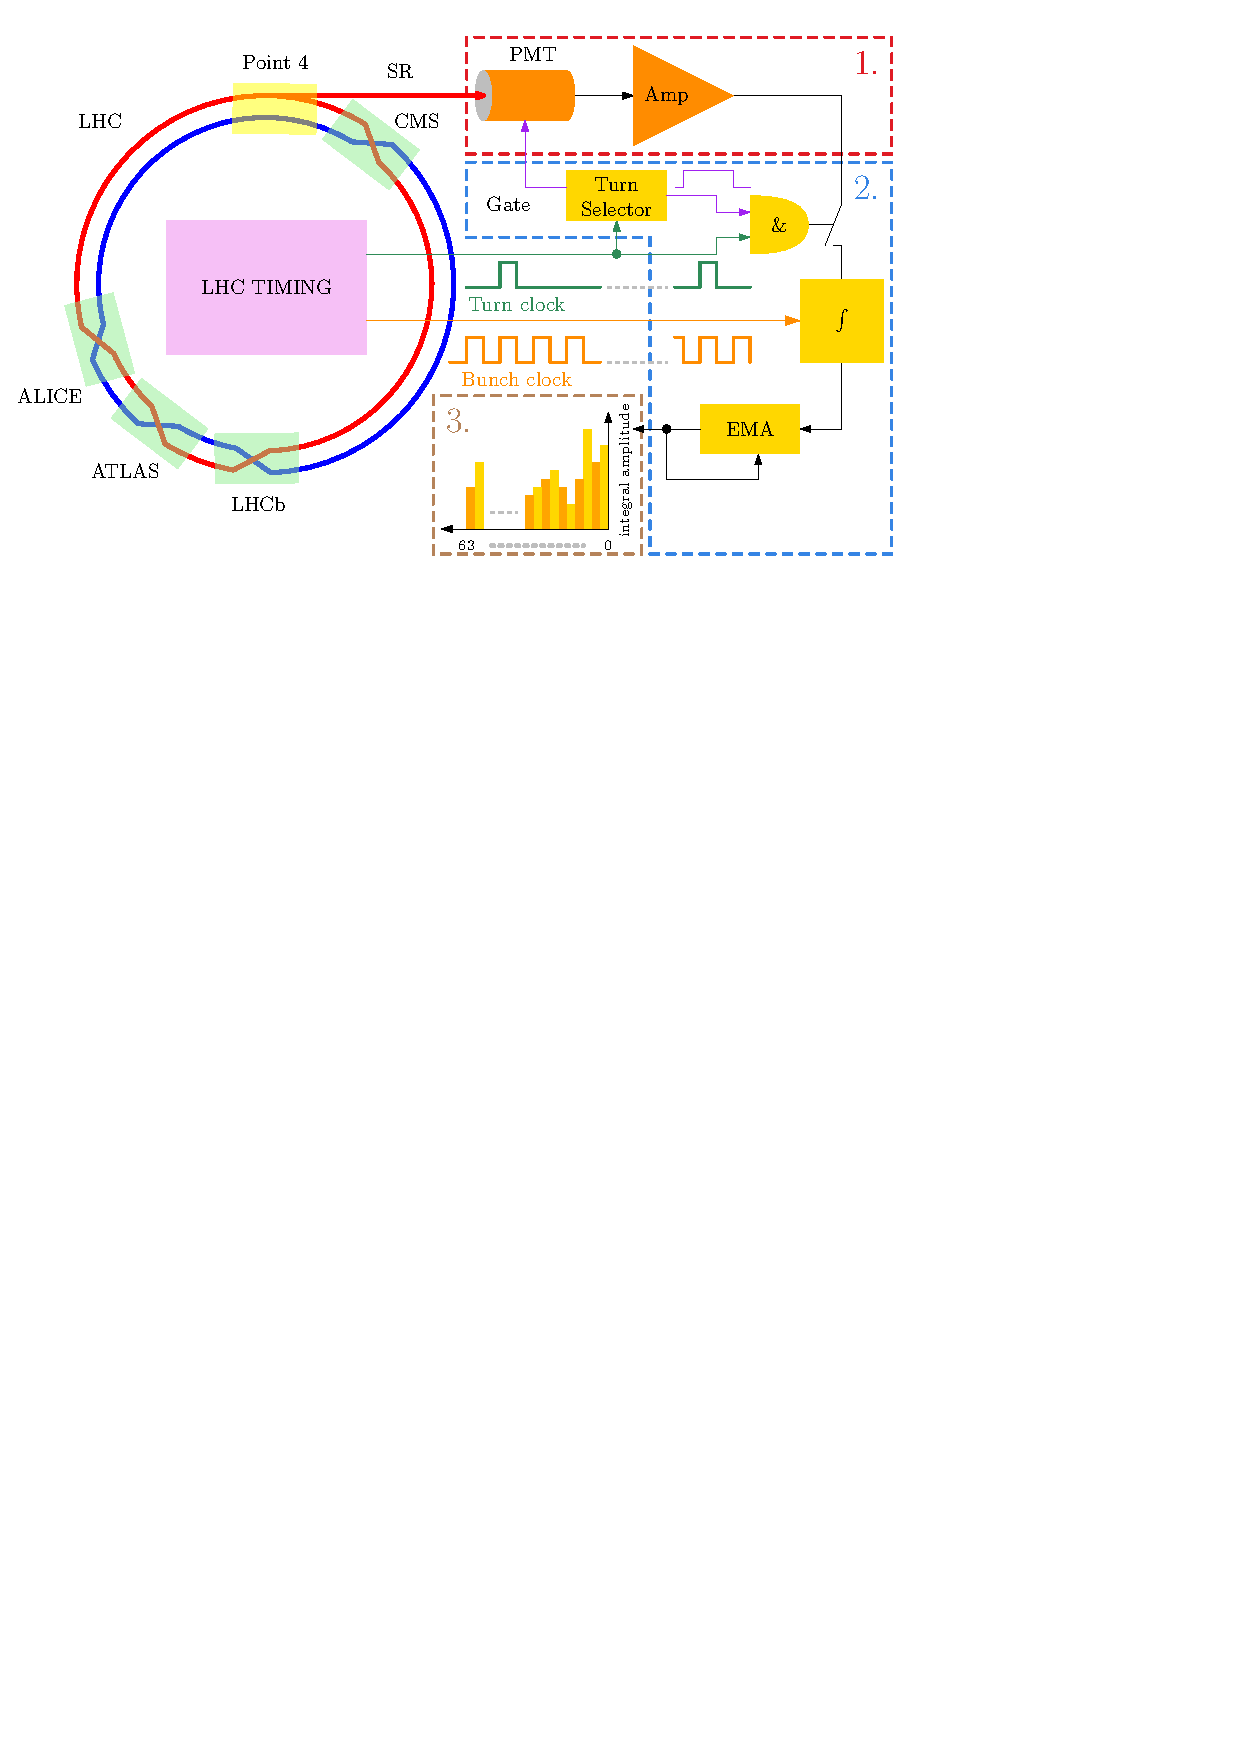
\includegraphics[width=\columnwidth]{bsra_chain.pdf}
    \caption{BSRA Chain}
    \label{fig:bsra_chain}
\end{figure} 
The diagram on the left depicts the layout of the LHC, with beam 1 represented
in red and beam 2 in blue. It includes all four experiments (Alice, Atlas,
LHCb, and CMS). The AGM is situated at Point 4 (indicated by the yellow
square), close to the CMS experiment. The Timing, Trigger, and Control system
(TTC) is shown as a purple rectangle in the center of the LHC ring. This system
receives RF clocking and broadcasts it as messages on the network (TTC
distribution)~\cite{ttc_distribution}. The AGM extracts bunch clock information
(corresponding to the position of bunches) and turn clock information (marking
the start of a turn) from these messages.\\
Beam intensity is gathered by measuring the synchrotron light (SL), as
indicated by the red line directed towards the Multi-channel photomultiplier
(MCP-PMT) in the optical front-end (OF). The beam traverses first optical
filters, which increase system dynamic range. Subsequently, the signal is
transmitted over a \SI{100}{m} cable. To compensate for losses in the cable,
the signal is amplified beforehand. It then proceeds to the Data Acquisition
(DAQ) system, which measures \SI{6.4}{\micro\second} window and integrates the
intervals of \SI{100}{\nano\second}. This creates set of 64 values published to
the SW every \SI{10}{\micro\second}.

\subsection{Working principle}
The measurement period is determined by the MCP-PMT used, which is the gated
HAMAMATSU R5916U-50 with a duty cycle of \SI{1}{\%}. With a gate pulse duration
of \SI{3}{\micro\second} and one turn cycle length of \SI{89}{\micro\second},
measurements are taken every 4th clock cycle (\SI{356}{\micro\second}),
reducing the duty cycle to \SI{0.84}{\%}.\\
The system captures 64 values with a granularity of \SI{100}{\nano\second}. The
MCP-PMT gate duration is \SI{3}{\micro\second} providing an additional degree of
freedom in system control. Each \SI{100}{\nano\second} value is averaged in an
extra EMA and provided to the software every \SI{100}{\micro\second}. This
time is enough to react to changes in AG. The population can change from
\SI{1.6}{\second} to \SI{25}{\second} due to different
effects~\cite{high_sensitivity_measurement}.

\subsection{Current Solution}
The current setup employs a DAB64x card with an FPGA Altera Stratix EP1S40 for
data processing. The platform features two FMC connectors, each hosting an IBMS
module integrating voltage input via the lhcb2002b ASIC~\cite{lhcb_asic}. To
maximize ADC resolution, the signal undergoes amplification using a HAMAMATSU
C5594 amplifier with a static gain of \SI{36}{dBV}, a bandwidth of
\SI{1.5}{GHz}, and a low cutoff frequency of \SI{50}{Hz}.
\begin{figure}[!tbh]
    \centering
    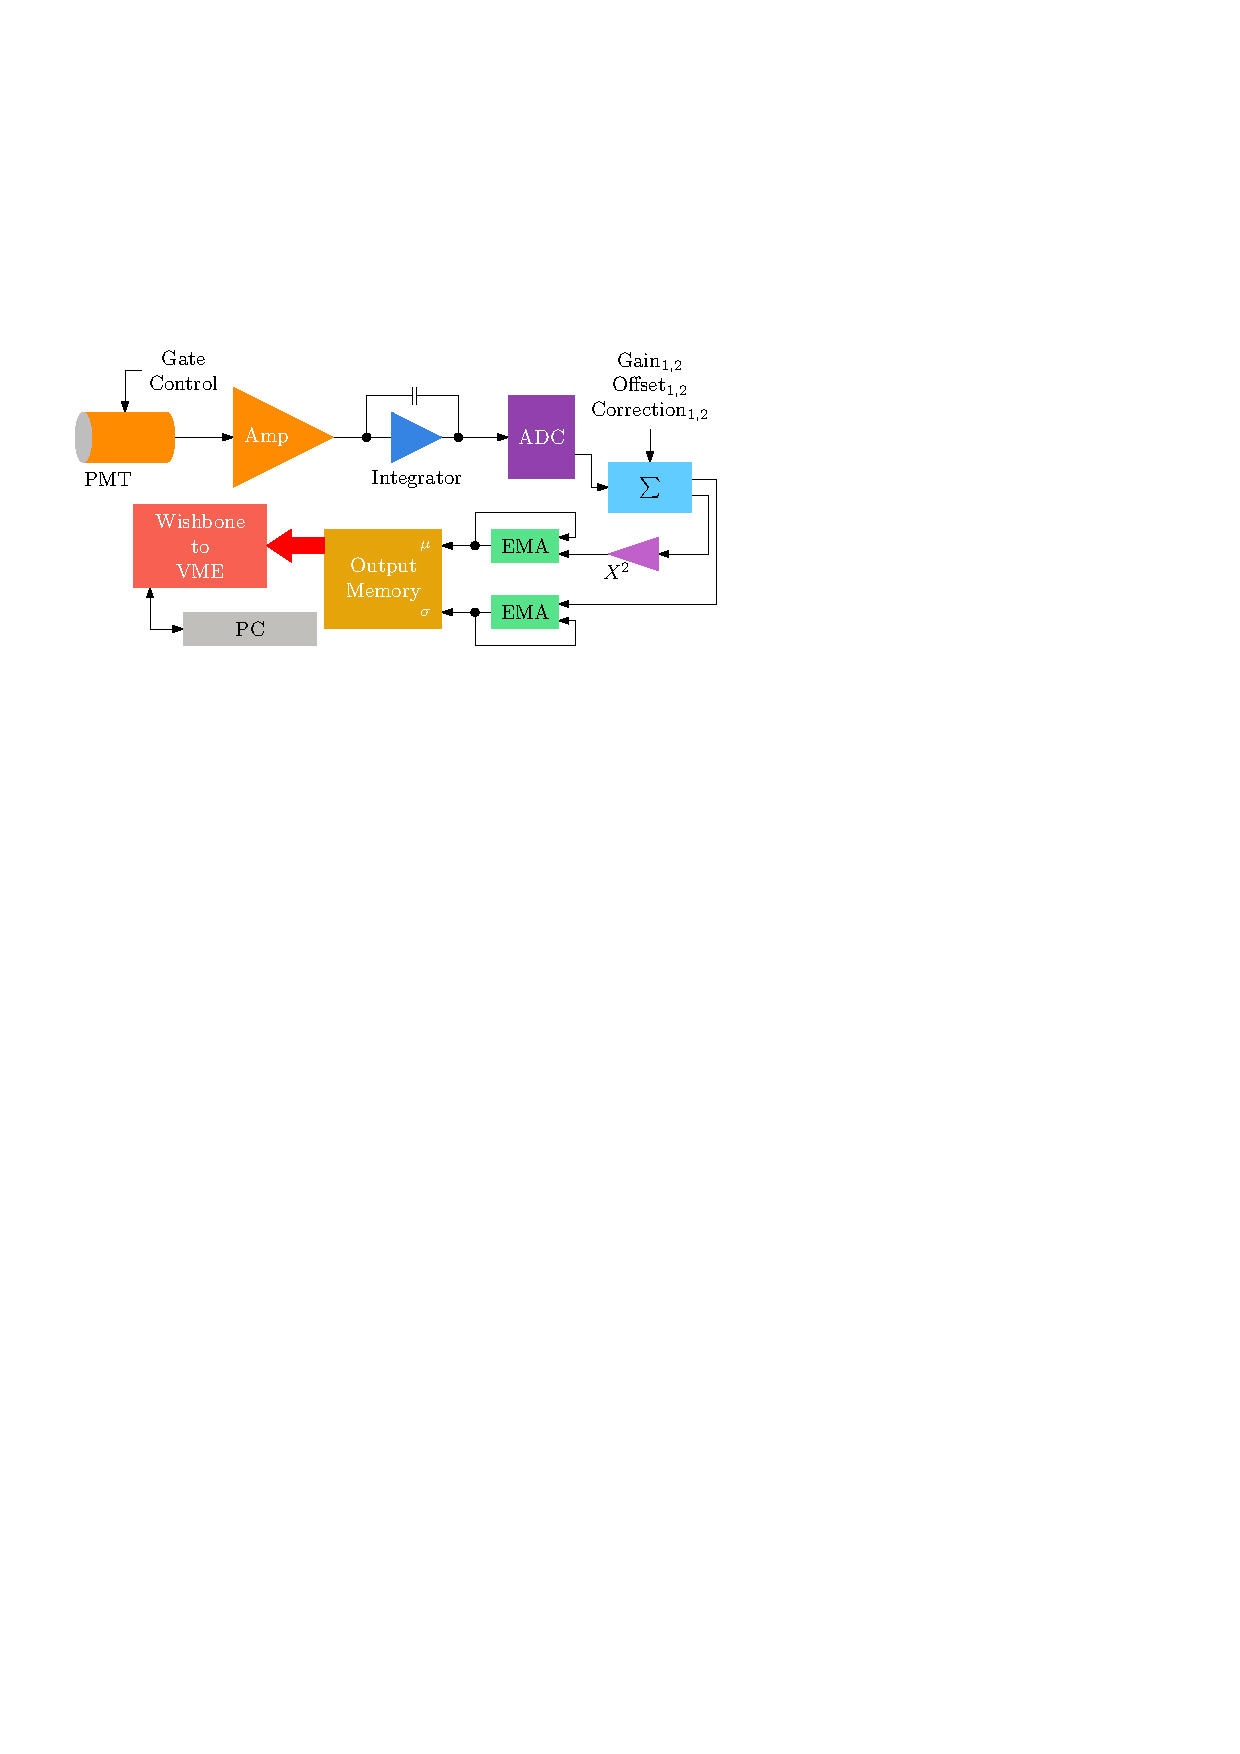
\includegraphics[width=\columnwidth]{existing_system_processing.pdf}
    \caption{Current system block diagram}
    \label{fig:current_system_processing}
\end{figure}
The system schematic is depicted in Fig.\ref{fig:current_system_processing}.
The OF remains consistent with the description provided
in the system architecture chapter. Notably, filters are not represented in the
image as they are universally applied. For optimal utilization of the \SI{40}{MHz}
ADC's full scale, the MCP-PMT signal necessitates a minimum amplification of
\SI{34}{dB}, a task accomplished by the Hamamatsu C559
amplifier\cite{bsra_first_operation}.\\
Within the schematic, the signal corresponding to a single bunch (\SI{25}{ns})
is integrated within the IBMS module (denoted by a blue triangle with a
capacitor in the feedback loop) and subsequently sampled by the ADC
(represented by a violet rectangle). The DAQ system integrates four samples
(indicated by a light blue rectangle with a $\sum$ symbol) to compute the
charge over a \SI{100}{ns} interval. This process generates 64 values, from
which two sets of 64 values are derived, encompassing the standard deviation
and mean value calculations. Both sets are then forwarded to the Exponential
Moving Average (EMA) block (depicted by a green rectangle). All collected data
are stored within the block RAM and subsequently shared with a PC via a
Wishbone to VME64 bridge. The PC operates a server, facilitating the FESA
interface for connected clients.

\subsection{Constraints and Limitations}
The present AGM exhibits artifacts in the measurements. Signals outside the
gating range do not exhibit the characteristics of white noise, attributed to
the lhcb2002b ASIC. The integrators' gain lacks linearity, featuring distinct
offsets and dead times. Consequently, the system necessitates correction for
these effects at each integrator, leading to uncertainties in the outcomes and
necessitating intricate calibration procedures.\\
The system relies on an outdated FPGA platform, rendering its development
software incompatible with the latest operating systems. Additionally, the
fixed amplifier configuration contributes to reduced resolution for signals of
smaller magnitudes.

\section{System Upgrade}
To address maintenance concerns, the VFC-HD carrier is employed alongside an
additional RTM board, facilitating gate driver functionality and control of the
built-in test LED. Leveraging the same carrier board equipped with a 500MSPS
14-bit ADC from previous projects meets the requirement for reducing
maintenance efforts. The updated system eliminates IBMS cards featuring
lhcb2002b integrators, transitioning the entire integration process to the
gateware.

\subsection{Low band Amplifier}
The newly developed custom amplifier is designed to accommodate a wider signal
dynamic range by virtue of its variability.
% A = U^2/(i^2 * R^2) => A_dB = 20*log10(U/(i*R))
Figure \ref{fig:amp_schematics} illustrates the block diagram of the amplifier.
All configurations are managed through a UART interface, facilitating
adjustments to the variable current-to-voltage conversion factor ranging from
\SI{5.8}{mV/\micro A} to \SI{1.1}{V/\micro A}. This corresponds to a voltage
gain range of \SI{41}{dB} to \SI{87}{dB}. The AGM ADC does not exhibit a zero
offset, allowing for signal shifting within the amplifier prior to
post-processing.\\
Additionally, the amplifier incorporates an alarm signal generator designed to
deactivate the gate when the incident light intensity exceeds safe levels,
potentially risking damage to the multi-channel plate within the PMT. The alarm
signal is transmitted to the gateware for processing and management. Notably,
the alarm feature includes a variable threshold setting.
\begin{figure}[!tbh]
    \centering
    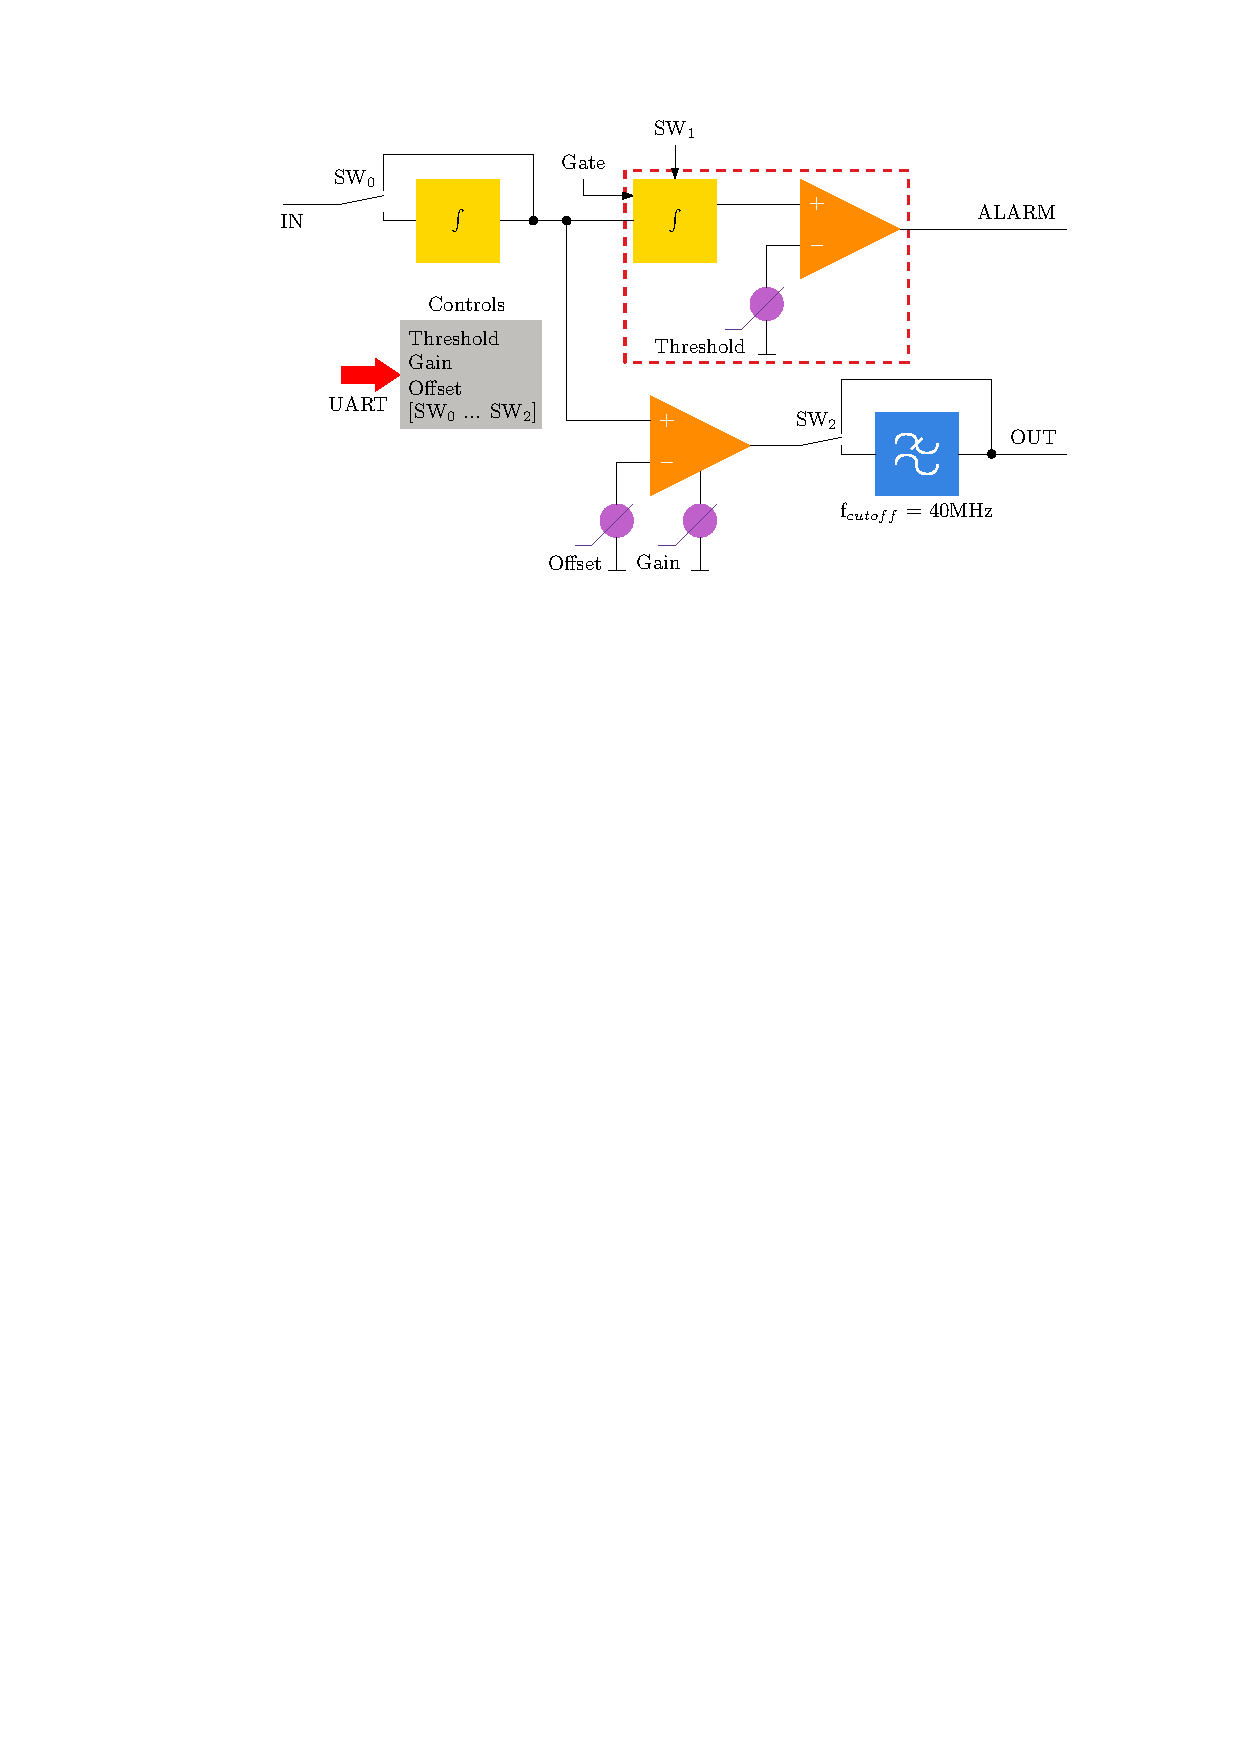
\includegraphics[width=\columnwidth]{amp_schematics.pdf}
    \caption{New AGM custom amplifier}
    \label{fig:amp_schematics}
\end{figure}
The amplifier design includes three switches. The first switch can configure
the pre-integrator to filter out spikes resulting from dark counts of the PMT.
The second switch enables selection between manual or gate-driven integration
of the acquisition window. The third switch activates low-pass filtering with a
cutoff frequency of \SI{40}{MHz}.

\subsection{Acquisition system}
The DAQ required redesigning for compatibility with the new VFC-HD carrier,
necessitating the integration of a Rear Transition Module (RTM) to facilitate
control of the gate and the built-in test LED. Figure~\ref{fig:bsra_daq}
illustrates the principle of DAQ functionality.
\begin{figure}[!tbh]
    \centering
    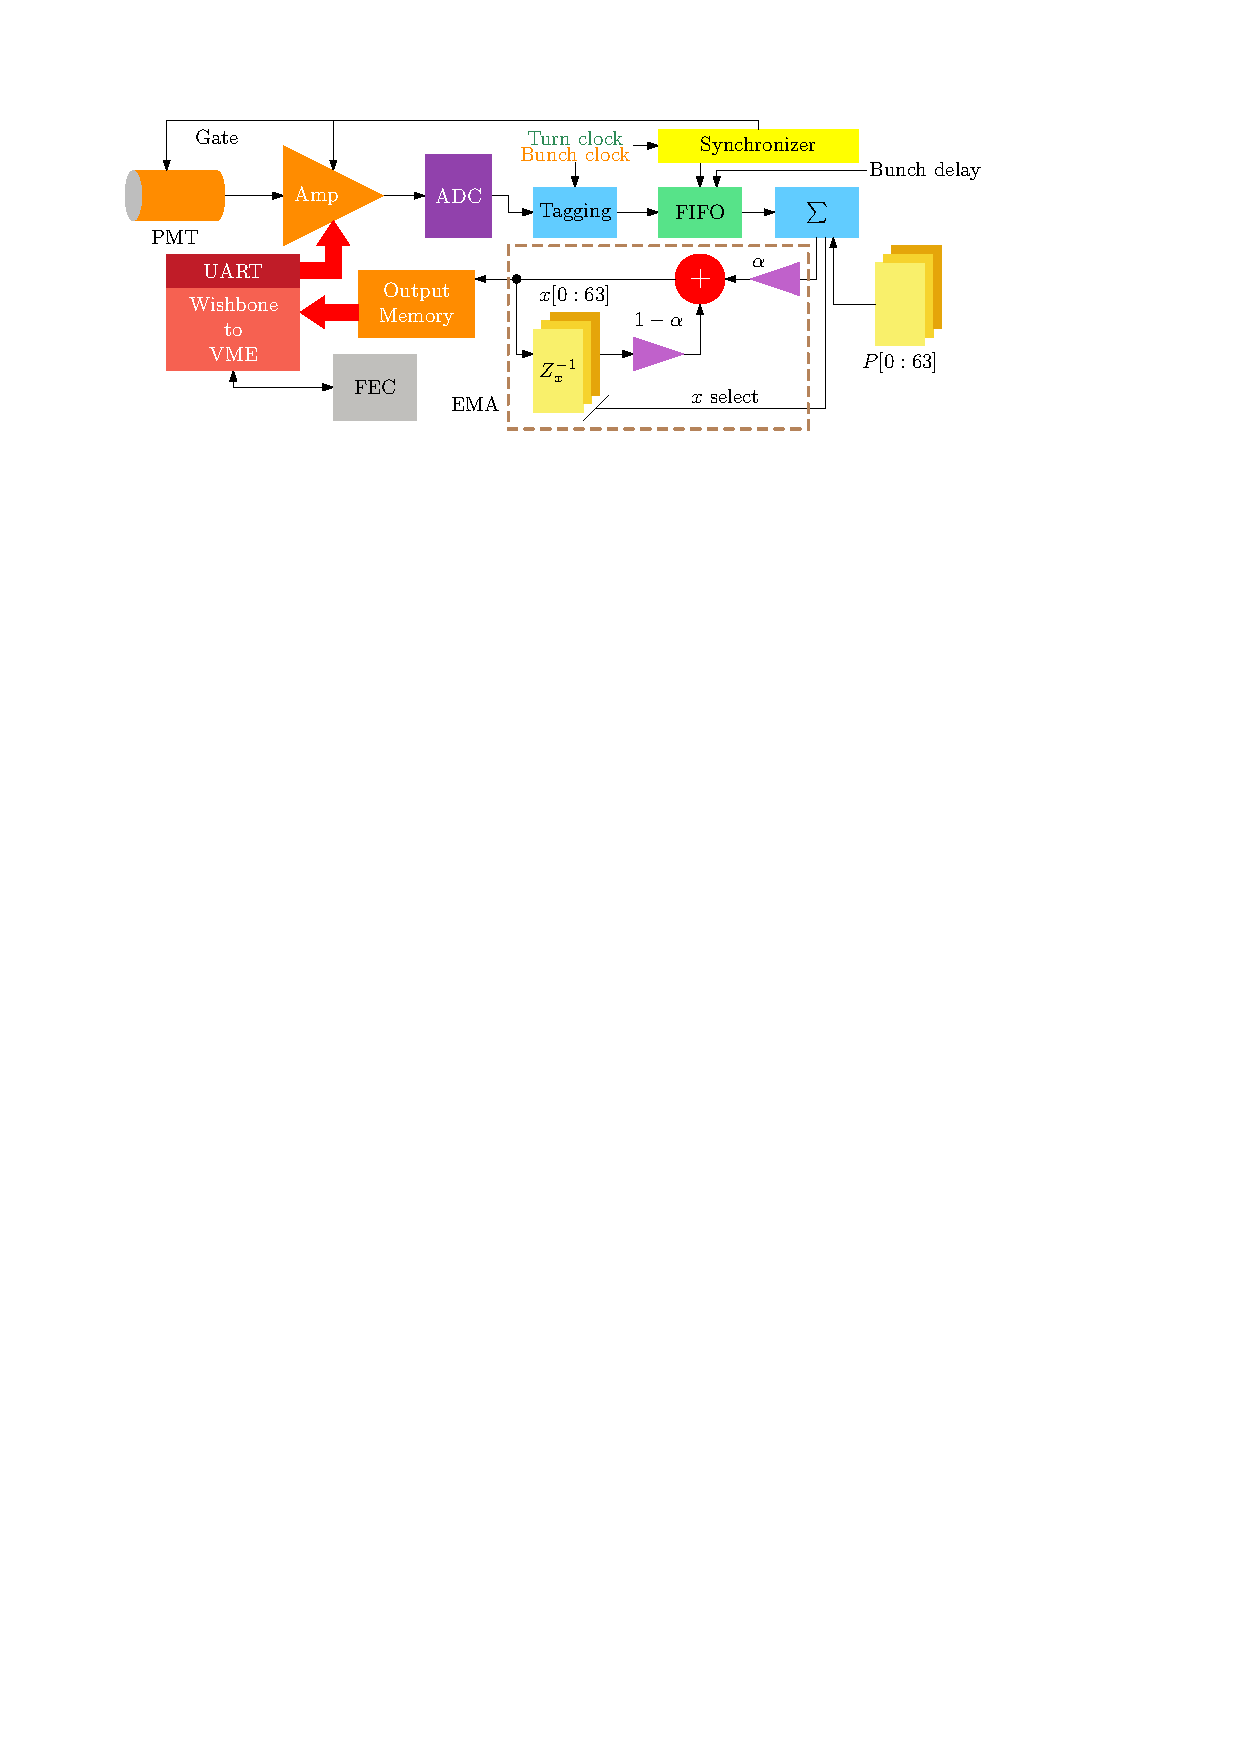
\includegraphics[width=\columnwidth]{bsra_daq.pdf}
    \caption{Ackquisition system schematics}
    \label{fig:bsra_daq}
\end{figure}
The new DAQ receives asynchronous data samples from a 500MSPS 14-bit ADC
(depicted as a violet rectangle), organized in blocks of four frames
every~\SI{8}{\nano s}, corresponding to one channel. Each frame contains 4 x
16-bit values. To compute integrals over~\SI{100}{\nano\second}, the system
employs data tagging. The tagging block resamples LHC timing at 500MSPS and
generates bunch and turn clock vector masks, storing information about both
clock phases. The 14-bit ADC data is left-aligned to 16-bit values. The tagger
sets the two least significant bits to one when the ADC sample falls within the
edge range.\\
The system stores data from the region of interest into a FIFO using the
synchronization block pulse. The stored data is then processed as a stream of
values passed to the integrator. The integrator begins summing values upon
encountering the tag indicating the start of the bunch, generating 64 values
offset from the pedestal memory (P[63:0]). This process subtracts accumulated
charge at the gate opening and closing edges. The resulting values are then
sent to the EMA, and the results are stored in the
block RAM accessible via the VME64x bus. The format of the data provided to the
PC via the running FESA server matches that of the current
AGM~\cite{my_thesis}.

\subsection{Installation in LHC}

The instrument OF and DAQ are situated in LHC Point 4 near the RF system. The
new installation is depicted in Fig.~\ref{fig:installation}, delineated by a
violet frame. Adjacent to its right side is the currently utilized AGM, while
the BSRS occupies the left side. All instruments share the same light source
with the BSRT. The instrument is extracted from the shielding, with the red
arrow indicating the direction from which light emanates and enters the MCP-PMT
of the new AGM.
\begin{figure}[!tbh]
    \centering
    \includegraphics[width=\columnwidth]{installation.jpg}
    \caption{New AGM installed in Point 4 next to BSRT}
    \label{fig:installation}
\end{figure}
Atop the reflective foil, which directs light towards the MCP-PMT, there's a
LED serving to simulate the light source, aiding in system verification. The
AGM amplifier is positioned atop the optical front-end for easy access during
interventions. To regulate light intensity, pneumatically controlled optical
filters are positioned in front of the MCP-PMT.

\section{Control Interface}
The gateware outputs data from four distinct block RAMs. The first RAM stores
raw data from the ADC, crucial for accurately setting the initial timing delay
of the instrument. It holds data for 1.5 turns, resulting in a publication rate
of~\SI{3.3}{Hz}. The subsequent two memories store both snapshot and averaged
data with finer granularity. They retain 10 samples per~\SI{10}{ms} window,
yielding a sample rate of~\SI{100}{Hz}. The final memory exclusively stores
averaged data collected every~\SI{10}{ms}, dictating the publication rate. Data
retrieval is managed by the FESA server, which receives interrupts whenever the
data becomes available.
\begin{figure}[!tbh]
    \centering
    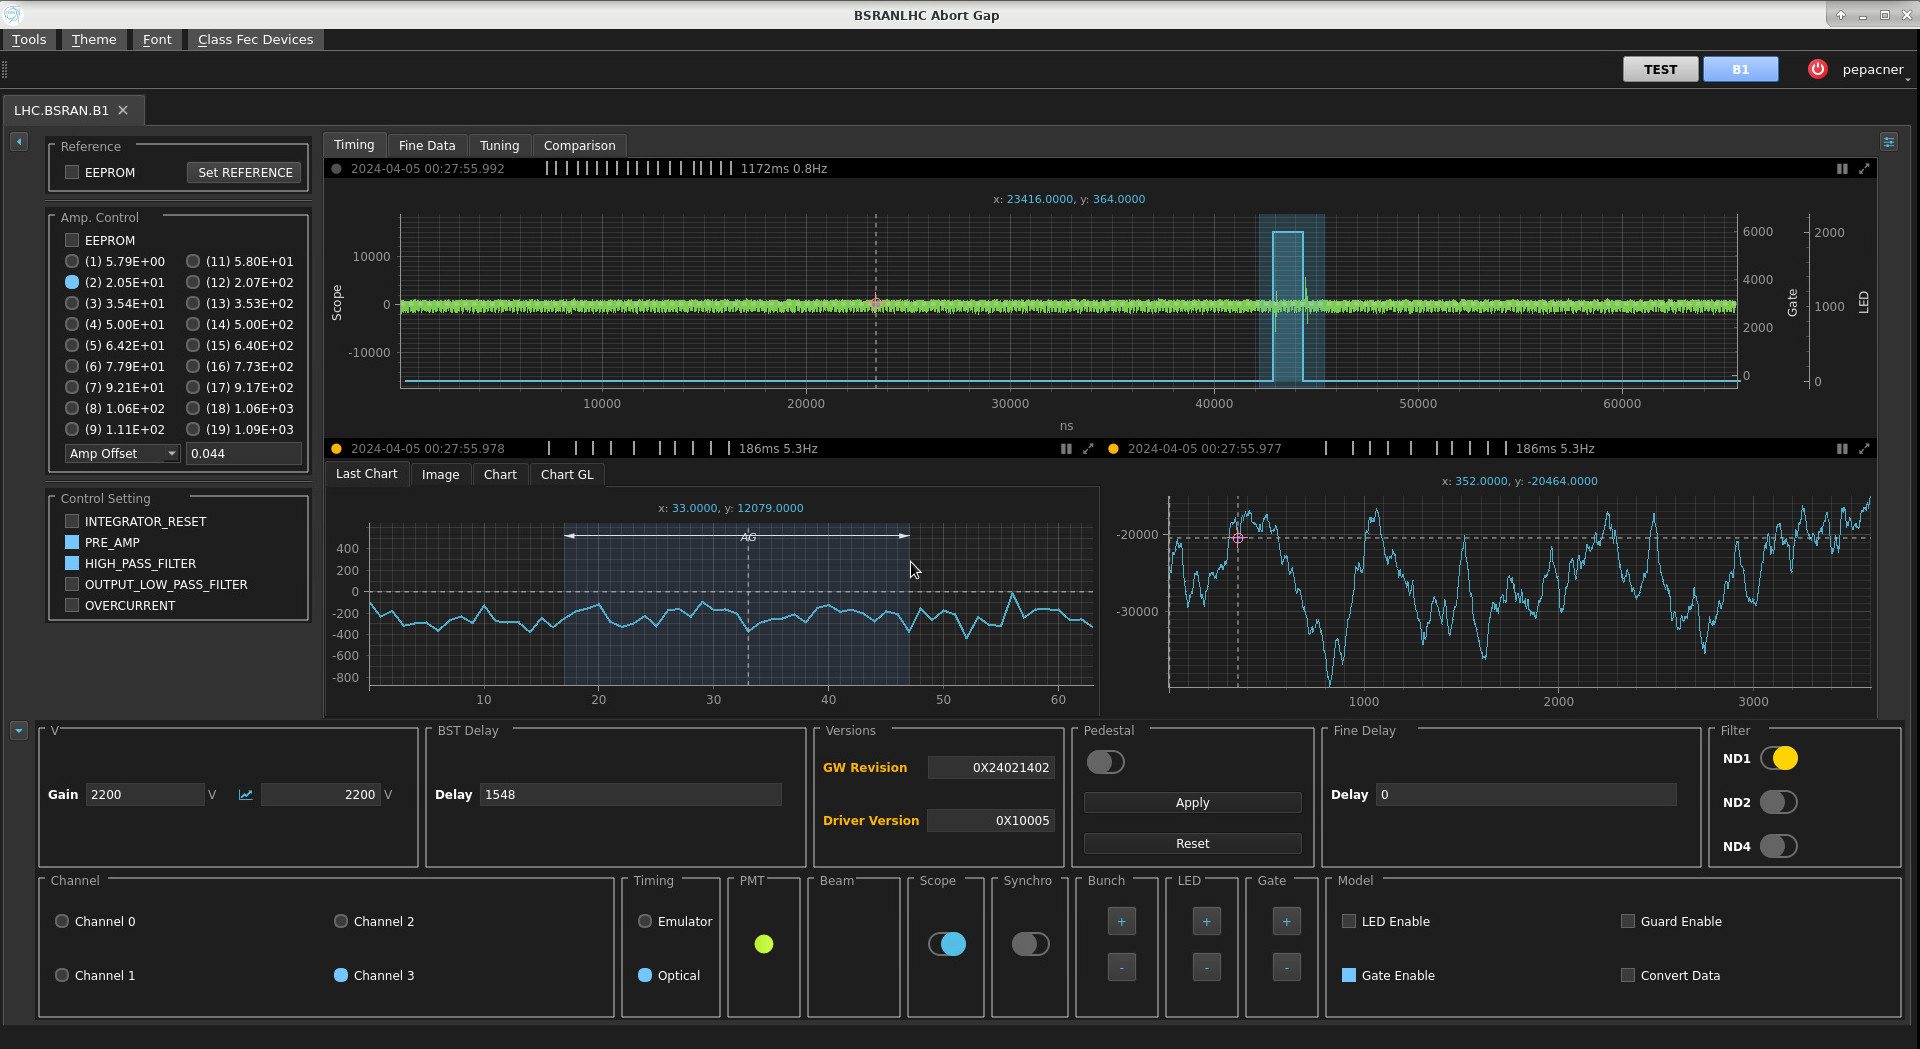
\includegraphics[width=\columnwidth]{control_interface.jpg}
    \caption{New AGM expert graphical interface}
    \label{fig:control_interface}
\end{figure}
To streamline setup tuning, a new interface was developed. Operating as a
client of the FESA server, it showcases the content of all block RAMs. The
primary control panel is illustrated in Fig.~\ref{fig:control_interface}. It
features three plots: raw data from the ADC (top plot), processed averaged data
(bottom-left plot), and the temporal evolution of the data (bottom-right plot).
The left menu governs amplifier settings, while the bottom menu regulates
acquisition delays and optical filters.

\section{First acquired plots}
The initial measurements were conducted in November 2023 using the ion beam.
The optical system divides the SL in a 1:8 ratio, resulting in significantly
less light reaching the new system compared to the current one. Consequently,
we anticipate lower deviation values for the system measuring light with higher
intensity.
\begin{figure}[!htb]
    \begin{center}
        \scalebox{0.54}{%% Creator: Matplotlib, PGF backend
%%
%% To include the figure in your LaTeX document, write
%%   \input{<filename>.pgf}
%%
%% Make sure the required packages are loaded in your preamble
%%   \usepackage{pgf}
%%
%% Also ensure that all the required font packages are loaded; for instance,
%% the lmodern package is sometimes necessary when using math font.
%%   \usepackage{lmodern}
%%
%% Figures using additional raster images can only be included by \input if
%% they are in the same directory as the main LaTeX file. For loading figures
%% from other directories you can use the `import` package
%%   \usepackage{import}
%%
%% and then include the figures with
%%   \import{<path to file>}{<filename>.pgf}
%%
%% Matplotlib used the following preamble
%%   \def\mathdefault#1{#1}
%%   \everymath=\expandafter{\the\everymath\displaystyle}
%%   
%%   \makeatletter\@ifpackageloaded{underscore}{}{\usepackage[strings]{underscore}}\makeatother
%%
\begingroup%
\makeatletter%
\begin{pgfpicture}%
\pgfpathrectangle{\pgfpointorigin}{\pgfqpoint{6.400000in}{4.800000in}}%
\pgfusepath{use as bounding box, clip}%
\begin{pgfscope}%
\pgfsetbuttcap%
\pgfsetmiterjoin%
\definecolor{currentfill}{rgb}{1.000000,1.000000,1.000000}%
\pgfsetfillcolor{currentfill}%
\pgfsetlinewidth{0.000000pt}%
\definecolor{currentstroke}{rgb}{1.000000,1.000000,1.000000}%
\pgfsetstrokecolor{currentstroke}%
\pgfsetdash{}{0pt}%
\pgfpathmoveto{\pgfqpoint{0.000000in}{0.000000in}}%
\pgfpathlineto{\pgfqpoint{6.400000in}{0.000000in}}%
\pgfpathlineto{\pgfqpoint{6.400000in}{4.800000in}}%
\pgfpathlineto{\pgfqpoint{0.000000in}{4.800000in}}%
\pgfpathlineto{\pgfqpoint{0.000000in}{0.000000in}}%
\pgfpathclose%
\pgfusepath{fill}%
\end{pgfscope}%
\begin{pgfscope}%
\pgfsetbuttcap%
\pgfsetmiterjoin%
\definecolor{currentfill}{rgb}{1.000000,1.000000,1.000000}%
\pgfsetfillcolor{currentfill}%
\pgfsetlinewidth{0.000000pt}%
\definecolor{currentstroke}{rgb}{0.000000,0.000000,0.000000}%
\pgfsetstrokecolor{currentstroke}%
\pgfsetstrokeopacity{0.000000}%
\pgfsetdash{}{0pt}%
\pgfpathmoveto{\pgfqpoint{0.800000in}{0.528000in}}%
\pgfpathlineto{\pgfqpoint{5.760000in}{0.528000in}}%
\pgfpathlineto{\pgfqpoint{5.760000in}{4.224000in}}%
\pgfpathlineto{\pgfqpoint{0.800000in}{4.224000in}}%
\pgfpathlineto{\pgfqpoint{0.800000in}{0.528000in}}%
\pgfpathclose%
\pgfusepath{fill}%
\end{pgfscope}%
\begin{pgfscope}%
\pgfpathrectangle{\pgfqpoint{0.800000in}{0.528000in}}{\pgfqpoint{4.960000in}{3.696000in}}%
\pgfusepath{clip}%
\pgfsetbuttcap%
\pgfsetroundjoin%
\pgfsetlinewidth{0.602250pt}%
\definecolor{currentstroke}{rgb}{0.700000,0.700000,0.700000}%
\pgfsetstrokecolor{currentstroke}%
\pgfsetdash{{2.220000pt}{0.960000pt}}{0.000000pt}%
\pgfpathmoveto{\pgfqpoint{0.800000in}{0.528000in}}%
\pgfpathlineto{\pgfqpoint{0.800000in}{4.224000in}}%
\pgfusepath{stroke}%
\end{pgfscope}%
\begin{pgfscope}%
\pgfsetbuttcap%
\pgfsetroundjoin%
\definecolor{currentfill}{rgb}{0.000000,0.000000,0.000000}%
\pgfsetfillcolor{currentfill}%
\pgfsetlinewidth{0.602250pt}%
\definecolor{currentstroke}{rgb}{0.000000,0.000000,0.000000}%
\pgfsetstrokecolor{currentstroke}%
\pgfsetdash{}{0pt}%
\pgfsys@defobject{currentmarker}{\pgfqpoint{0.000000in}{0.000000in}}{\pgfqpoint{0.000000in}{0.048611in}}{%
\pgfpathmoveto{\pgfqpoint{0.000000in}{0.000000in}}%
\pgfpathlineto{\pgfqpoint{0.000000in}{0.048611in}}%
\pgfusepath{stroke,fill}%
}%
\begin{pgfscope}%
\pgfsys@transformshift{0.800000in}{0.528000in}%
\pgfsys@useobject{currentmarker}{}%
\end{pgfscope}%
\end{pgfscope}%
\begin{pgfscope}%
\pgfsetbuttcap%
\pgfsetroundjoin%
\definecolor{currentfill}{rgb}{0.000000,0.000000,0.000000}%
\pgfsetfillcolor{currentfill}%
\pgfsetlinewidth{0.602250pt}%
\definecolor{currentstroke}{rgb}{0.000000,0.000000,0.000000}%
\pgfsetstrokecolor{currentstroke}%
\pgfsetdash{}{0pt}%
\pgfsys@defobject{currentmarker}{\pgfqpoint{0.000000in}{-0.048611in}}{\pgfqpoint{0.000000in}{0.000000in}}{%
\pgfpathmoveto{\pgfqpoint{0.000000in}{0.000000in}}%
\pgfpathlineto{\pgfqpoint{0.000000in}{-0.048611in}}%
\pgfusepath{stroke,fill}%
}%
\begin{pgfscope}%
\pgfsys@transformshift{0.800000in}{4.224000in}%
\pgfsys@useobject{currentmarker}{}%
\end{pgfscope}%
\end{pgfscope}%
\begin{pgfscope}%
\definecolor{textcolor}{rgb}{0.000000,0.000000,0.000000}%
\pgfsetstrokecolor{textcolor}%
\pgfsetfillcolor{textcolor}%
\pgftext[x=0.800000in,y=0.479389in,,top]{\color{textcolor}{\rmfamily\fontsize{8.330000}{9.996000}\selectfont\catcode`\^=\active\def^{\ifmmode\sp\else\^{}\fi}\catcode`\%=\active\def%{\%}$\mathdefault{0}$}}%
\end{pgfscope}%
\begin{pgfscope}%
\pgfpathrectangle{\pgfqpoint{0.800000in}{0.528000in}}{\pgfqpoint{4.960000in}{3.696000in}}%
\pgfusepath{clip}%
\pgfsetbuttcap%
\pgfsetroundjoin%
\pgfsetlinewidth{0.602250pt}%
\definecolor{currentstroke}{rgb}{0.700000,0.700000,0.700000}%
\pgfsetstrokecolor{currentstroke}%
\pgfsetdash{{2.220000pt}{0.960000pt}}{0.000000pt}%
\pgfpathmoveto{\pgfqpoint{1.508571in}{0.528000in}}%
\pgfpathlineto{\pgfqpoint{1.508571in}{4.224000in}}%
\pgfusepath{stroke}%
\end{pgfscope}%
\begin{pgfscope}%
\pgfsetbuttcap%
\pgfsetroundjoin%
\definecolor{currentfill}{rgb}{0.000000,0.000000,0.000000}%
\pgfsetfillcolor{currentfill}%
\pgfsetlinewidth{0.602250pt}%
\definecolor{currentstroke}{rgb}{0.000000,0.000000,0.000000}%
\pgfsetstrokecolor{currentstroke}%
\pgfsetdash{}{0pt}%
\pgfsys@defobject{currentmarker}{\pgfqpoint{0.000000in}{0.000000in}}{\pgfqpoint{0.000000in}{0.048611in}}{%
\pgfpathmoveto{\pgfqpoint{0.000000in}{0.000000in}}%
\pgfpathlineto{\pgfqpoint{0.000000in}{0.048611in}}%
\pgfusepath{stroke,fill}%
}%
\begin{pgfscope}%
\pgfsys@transformshift{1.508571in}{0.528000in}%
\pgfsys@useobject{currentmarker}{}%
\end{pgfscope}%
\end{pgfscope}%
\begin{pgfscope}%
\pgfsetbuttcap%
\pgfsetroundjoin%
\definecolor{currentfill}{rgb}{0.000000,0.000000,0.000000}%
\pgfsetfillcolor{currentfill}%
\pgfsetlinewidth{0.602250pt}%
\definecolor{currentstroke}{rgb}{0.000000,0.000000,0.000000}%
\pgfsetstrokecolor{currentstroke}%
\pgfsetdash{}{0pt}%
\pgfsys@defobject{currentmarker}{\pgfqpoint{0.000000in}{-0.048611in}}{\pgfqpoint{0.000000in}{0.000000in}}{%
\pgfpathmoveto{\pgfqpoint{0.000000in}{0.000000in}}%
\pgfpathlineto{\pgfqpoint{0.000000in}{-0.048611in}}%
\pgfusepath{stroke,fill}%
}%
\begin{pgfscope}%
\pgfsys@transformshift{1.508571in}{4.224000in}%
\pgfsys@useobject{currentmarker}{}%
\end{pgfscope}%
\end{pgfscope}%
\begin{pgfscope}%
\definecolor{textcolor}{rgb}{0.000000,0.000000,0.000000}%
\pgfsetstrokecolor{textcolor}%
\pgfsetfillcolor{textcolor}%
\pgftext[x=1.508571in,y=0.479389in,,top]{\color{textcolor}{\rmfamily\fontsize{8.330000}{9.996000}\selectfont\catcode`\^=\active\def^{\ifmmode\sp\else\^{}\fi}\catcode`\%=\active\def%{\%}$\mathdefault{9}$}}%
\end{pgfscope}%
\begin{pgfscope}%
\pgfpathrectangle{\pgfqpoint{0.800000in}{0.528000in}}{\pgfqpoint{4.960000in}{3.696000in}}%
\pgfusepath{clip}%
\pgfsetbuttcap%
\pgfsetroundjoin%
\pgfsetlinewidth{0.602250pt}%
\definecolor{currentstroke}{rgb}{0.700000,0.700000,0.700000}%
\pgfsetstrokecolor{currentstroke}%
\pgfsetdash{{2.220000pt}{0.960000pt}}{0.000000pt}%
\pgfpathmoveto{\pgfqpoint{2.217143in}{0.528000in}}%
\pgfpathlineto{\pgfqpoint{2.217143in}{4.224000in}}%
\pgfusepath{stroke}%
\end{pgfscope}%
\begin{pgfscope}%
\pgfsetbuttcap%
\pgfsetroundjoin%
\definecolor{currentfill}{rgb}{0.000000,0.000000,0.000000}%
\pgfsetfillcolor{currentfill}%
\pgfsetlinewidth{0.602250pt}%
\definecolor{currentstroke}{rgb}{0.000000,0.000000,0.000000}%
\pgfsetstrokecolor{currentstroke}%
\pgfsetdash{}{0pt}%
\pgfsys@defobject{currentmarker}{\pgfqpoint{0.000000in}{0.000000in}}{\pgfqpoint{0.000000in}{0.048611in}}{%
\pgfpathmoveto{\pgfqpoint{0.000000in}{0.000000in}}%
\pgfpathlineto{\pgfqpoint{0.000000in}{0.048611in}}%
\pgfusepath{stroke,fill}%
}%
\begin{pgfscope}%
\pgfsys@transformshift{2.217143in}{0.528000in}%
\pgfsys@useobject{currentmarker}{}%
\end{pgfscope}%
\end{pgfscope}%
\begin{pgfscope}%
\pgfsetbuttcap%
\pgfsetroundjoin%
\definecolor{currentfill}{rgb}{0.000000,0.000000,0.000000}%
\pgfsetfillcolor{currentfill}%
\pgfsetlinewidth{0.602250pt}%
\definecolor{currentstroke}{rgb}{0.000000,0.000000,0.000000}%
\pgfsetstrokecolor{currentstroke}%
\pgfsetdash{}{0pt}%
\pgfsys@defobject{currentmarker}{\pgfqpoint{0.000000in}{-0.048611in}}{\pgfqpoint{0.000000in}{0.000000in}}{%
\pgfpathmoveto{\pgfqpoint{0.000000in}{0.000000in}}%
\pgfpathlineto{\pgfqpoint{0.000000in}{-0.048611in}}%
\pgfusepath{stroke,fill}%
}%
\begin{pgfscope}%
\pgfsys@transformshift{2.217143in}{4.224000in}%
\pgfsys@useobject{currentmarker}{}%
\end{pgfscope}%
\end{pgfscope}%
\begin{pgfscope}%
\definecolor{textcolor}{rgb}{0.000000,0.000000,0.000000}%
\pgfsetstrokecolor{textcolor}%
\pgfsetfillcolor{textcolor}%
\pgftext[x=2.217143in,y=0.479389in,,top]{\color{textcolor}{\rmfamily\fontsize{8.330000}{9.996000}\selectfont\catcode`\^=\active\def^{\ifmmode\sp\else\^{}\fi}\catcode`\%=\active\def%{\%}$\mathdefault{18}$}}%
\end{pgfscope}%
\begin{pgfscope}%
\pgfpathrectangle{\pgfqpoint{0.800000in}{0.528000in}}{\pgfqpoint{4.960000in}{3.696000in}}%
\pgfusepath{clip}%
\pgfsetbuttcap%
\pgfsetroundjoin%
\pgfsetlinewidth{0.602250pt}%
\definecolor{currentstroke}{rgb}{0.700000,0.700000,0.700000}%
\pgfsetstrokecolor{currentstroke}%
\pgfsetdash{{2.220000pt}{0.960000pt}}{0.000000pt}%
\pgfpathmoveto{\pgfqpoint{2.925714in}{0.528000in}}%
\pgfpathlineto{\pgfqpoint{2.925714in}{4.224000in}}%
\pgfusepath{stroke}%
\end{pgfscope}%
\begin{pgfscope}%
\pgfsetbuttcap%
\pgfsetroundjoin%
\definecolor{currentfill}{rgb}{0.000000,0.000000,0.000000}%
\pgfsetfillcolor{currentfill}%
\pgfsetlinewidth{0.602250pt}%
\definecolor{currentstroke}{rgb}{0.000000,0.000000,0.000000}%
\pgfsetstrokecolor{currentstroke}%
\pgfsetdash{}{0pt}%
\pgfsys@defobject{currentmarker}{\pgfqpoint{0.000000in}{0.000000in}}{\pgfqpoint{0.000000in}{0.048611in}}{%
\pgfpathmoveto{\pgfqpoint{0.000000in}{0.000000in}}%
\pgfpathlineto{\pgfqpoint{0.000000in}{0.048611in}}%
\pgfusepath{stroke,fill}%
}%
\begin{pgfscope}%
\pgfsys@transformshift{2.925714in}{0.528000in}%
\pgfsys@useobject{currentmarker}{}%
\end{pgfscope}%
\end{pgfscope}%
\begin{pgfscope}%
\pgfsetbuttcap%
\pgfsetroundjoin%
\definecolor{currentfill}{rgb}{0.000000,0.000000,0.000000}%
\pgfsetfillcolor{currentfill}%
\pgfsetlinewidth{0.602250pt}%
\definecolor{currentstroke}{rgb}{0.000000,0.000000,0.000000}%
\pgfsetstrokecolor{currentstroke}%
\pgfsetdash{}{0pt}%
\pgfsys@defobject{currentmarker}{\pgfqpoint{0.000000in}{-0.048611in}}{\pgfqpoint{0.000000in}{0.000000in}}{%
\pgfpathmoveto{\pgfqpoint{0.000000in}{0.000000in}}%
\pgfpathlineto{\pgfqpoint{0.000000in}{-0.048611in}}%
\pgfusepath{stroke,fill}%
}%
\begin{pgfscope}%
\pgfsys@transformshift{2.925714in}{4.224000in}%
\pgfsys@useobject{currentmarker}{}%
\end{pgfscope}%
\end{pgfscope}%
\begin{pgfscope}%
\definecolor{textcolor}{rgb}{0.000000,0.000000,0.000000}%
\pgfsetstrokecolor{textcolor}%
\pgfsetfillcolor{textcolor}%
\pgftext[x=2.925714in,y=0.479389in,,top]{\color{textcolor}{\rmfamily\fontsize{8.330000}{9.996000}\selectfont\catcode`\^=\active\def^{\ifmmode\sp\else\^{}\fi}\catcode`\%=\active\def%{\%}$\mathdefault{27}$}}%
\end{pgfscope}%
\begin{pgfscope}%
\pgfpathrectangle{\pgfqpoint{0.800000in}{0.528000in}}{\pgfqpoint{4.960000in}{3.696000in}}%
\pgfusepath{clip}%
\pgfsetbuttcap%
\pgfsetroundjoin%
\pgfsetlinewidth{0.602250pt}%
\definecolor{currentstroke}{rgb}{0.700000,0.700000,0.700000}%
\pgfsetstrokecolor{currentstroke}%
\pgfsetdash{{2.220000pt}{0.960000pt}}{0.000000pt}%
\pgfpathmoveto{\pgfqpoint{3.634286in}{0.528000in}}%
\pgfpathlineto{\pgfqpoint{3.634286in}{4.224000in}}%
\pgfusepath{stroke}%
\end{pgfscope}%
\begin{pgfscope}%
\pgfsetbuttcap%
\pgfsetroundjoin%
\definecolor{currentfill}{rgb}{0.000000,0.000000,0.000000}%
\pgfsetfillcolor{currentfill}%
\pgfsetlinewidth{0.602250pt}%
\definecolor{currentstroke}{rgb}{0.000000,0.000000,0.000000}%
\pgfsetstrokecolor{currentstroke}%
\pgfsetdash{}{0pt}%
\pgfsys@defobject{currentmarker}{\pgfqpoint{0.000000in}{0.000000in}}{\pgfqpoint{0.000000in}{0.048611in}}{%
\pgfpathmoveto{\pgfqpoint{0.000000in}{0.000000in}}%
\pgfpathlineto{\pgfqpoint{0.000000in}{0.048611in}}%
\pgfusepath{stroke,fill}%
}%
\begin{pgfscope}%
\pgfsys@transformshift{3.634286in}{0.528000in}%
\pgfsys@useobject{currentmarker}{}%
\end{pgfscope}%
\end{pgfscope}%
\begin{pgfscope}%
\pgfsetbuttcap%
\pgfsetroundjoin%
\definecolor{currentfill}{rgb}{0.000000,0.000000,0.000000}%
\pgfsetfillcolor{currentfill}%
\pgfsetlinewidth{0.602250pt}%
\definecolor{currentstroke}{rgb}{0.000000,0.000000,0.000000}%
\pgfsetstrokecolor{currentstroke}%
\pgfsetdash{}{0pt}%
\pgfsys@defobject{currentmarker}{\pgfqpoint{0.000000in}{-0.048611in}}{\pgfqpoint{0.000000in}{0.000000in}}{%
\pgfpathmoveto{\pgfqpoint{0.000000in}{0.000000in}}%
\pgfpathlineto{\pgfqpoint{0.000000in}{-0.048611in}}%
\pgfusepath{stroke,fill}%
}%
\begin{pgfscope}%
\pgfsys@transformshift{3.634286in}{4.224000in}%
\pgfsys@useobject{currentmarker}{}%
\end{pgfscope}%
\end{pgfscope}%
\begin{pgfscope}%
\definecolor{textcolor}{rgb}{0.000000,0.000000,0.000000}%
\pgfsetstrokecolor{textcolor}%
\pgfsetfillcolor{textcolor}%
\pgftext[x=3.634286in,y=0.479389in,,top]{\color{textcolor}{\rmfamily\fontsize{8.330000}{9.996000}\selectfont\catcode`\^=\active\def^{\ifmmode\sp\else\^{}\fi}\catcode`\%=\active\def%{\%}$\mathdefault{36}$}}%
\end{pgfscope}%
\begin{pgfscope}%
\pgfpathrectangle{\pgfqpoint{0.800000in}{0.528000in}}{\pgfqpoint{4.960000in}{3.696000in}}%
\pgfusepath{clip}%
\pgfsetbuttcap%
\pgfsetroundjoin%
\pgfsetlinewidth{0.602250pt}%
\definecolor{currentstroke}{rgb}{0.700000,0.700000,0.700000}%
\pgfsetstrokecolor{currentstroke}%
\pgfsetdash{{2.220000pt}{0.960000pt}}{0.000000pt}%
\pgfpathmoveto{\pgfqpoint{4.342857in}{0.528000in}}%
\pgfpathlineto{\pgfqpoint{4.342857in}{4.224000in}}%
\pgfusepath{stroke}%
\end{pgfscope}%
\begin{pgfscope}%
\pgfsetbuttcap%
\pgfsetroundjoin%
\definecolor{currentfill}{rgb}{0.000000,0.000000,0.000000}%
\pgfsetfillcolor{currentfill}%
\pgfsetlinewidth{0.602250pt}%
\definecolor{currentstroke}{rgb}{0.000000,0.000000,0.000000}%
\pgfsetstrokecolor{currentstroke}%
\pgfsetdash{}{0pt}%
\pgfsys@defobject{currentmarker}{\pgfqpoint{0.000000in}{0.000000in}}{\pgfqpoint{0.000000in}{0.048611in}}{%
\pgfpathmoveto{\pgfqpoint{0.000000in}{0.000000in}}%
\pgfpathlineto{\pgfqpoint{0.000000in}{0.048611in}}%
\pgfusepath{stroke,fill}%
}%
\begin{pgfscope}%
\pgfsys@transformshift{4.342857in}{0.528000in}%
\pgfsys@useobject{currentmarker}{}%
\end{pgfscope}%
\end{pgfscope}%
\begin{pgfscope}%
\pgfsetbuttcap%
\pgfsetroundjoin%
\definecolor{currentfill}{rgb}{0.000000,0.000000,0.000000}%
\pgfsetfillcolor{currentfill}%
\pgfsetlinewidth{0.602250pt}%
\definecolor{currentstroke}{rgb}{0.000000,0.000000,0.000000}%
\pgfsetstrokecolor{currentstroke}%
\pgfsetdash{}{0pt}%
\pgfsys@defobject{currentmarker}{\pgfqpoint{0.000000in}{-0.048611in}}{\pgfqpoint{0.000000in}{0.000000in}}{%
\pgfpathmoveto{\pgfqpoint{0.000000in}{0.000000in}}%
\pgfpathlineto{\pgfqpoint{0.000000in}{-0.048611in}}%
\pgfusepath{stroke,fill}%
}%
\begin{pgfscope}%
\pgfsys@transformshift{4.342857in}{4.224000in}%
\pgfsys@useobject{currentmarker}{}%
\end{pgfscope}%
\end{pgfscope}%
\begin{pgfscope}%
\definecolor{textcolor}{rgb}{0.000000,0.000000,0.000000}%
\pgfsetstrokecolor{textcolor}%
\pgfsetfillcolor{textcolor}%
\pgftext[x=4.342857in,y=0.479389in,,top]{\color{textcolor}{\rmfamily\fontsize{8.330000}{9.996000}\selectfont\catcode`\^=\active\def^{\ifmmode\sp\else\^{}\fi}\catcode`\%=\active\def%{\%}$\mathdefault{45}$}}%
\end{pgfscope}%
\begin{pgfscope}%
\pgfpathrectangle{\pgfqpoint{0.800000in}{0.528000in}}{\pgfqpoint{4.960000in}{3.696000in}}%
\pgfusepath{clip}%
\pgfsetbuttcap%
\pgfsetroundjoin%
\pgfsetlinewidth{0.602250pt}%
\definecolor{currentstroke}{rgb}{0.700000,0.700000,0.700000}%
\pgfsetstrokecolor{currentstroke}%
\pgfsetdash{{2.220000pt}{0.960000pt}}{0.000000pt}%
\pgfpathmoveto{\pgfqpoint{5.051429in}{0.528000in}}%
\pgfpathlineto{\pgfqpoint{5.051429in}{4.224000in}}%
\pgfusepath{stroke}%
\end{pgfscope}%
\begin{pgfscope}%
\pgfsetbuttcap%
\pgfsetroundjoin%
\definecolor{currentfill}{rgb}{0.000000,0.000000,0.000000}%
\pgfsetfillcolor{currentfill}%
\pgfsetlinewidth{0.602250pt}%
\definecolor{currentstroke}{rgb}{0.000000,0.000000,0.000000}%
\pgfsetstrokecolor{currentstroke}%
\pgfsetdash{}{0pt}%
\pgfsys@defobject{currentmarker}{\pgfqpoint{0.000000in}{0.000000in}}{\pgfqpoint{0.000000in}{0.048611in}}{%
\pgfpathmoveto{\pgfqpoint{0.000000in}{0.000000in}}%
\pgfpathlineto{\pgfqpoint{0.000000in}{0.048611in}}%
\pgfusepath{stroke,fill}%
}%
\begin{pgfscope}%
\pgfsys@transformshift{5.051429in}{0.528000in}%
\pgfsys@useobject{currentmarker}{}%
\end{pgfscope}%
\end{pgfscope}%
\begin{pgfscope}%
\pgfsetbuttcap%
\pgfsetroundjoin%
\definecolor{currentfill}{rgb}{0.000000,0.000000,0.000000}%
\pgfsetfillcolor{currentfill}%
\pgfsetlinewidth{0.602250pt}%
\definecolor{currentstroke}{rgb}{0.000000,0.000000,0.000000}%
\pgfsetstrokecolor{currentstroke}%
\pgfsetdash{}{0pt}%
\pgfsys@defobject{currentmarker}{\pgfqpoint{0.000000in}{-0.048611in}}{\pgfqpoint{0.000000in}{0.000000in}}{%
\pgfpathmoveto{\pgfqpoint{0.000000in}{0.000000in}}%
\pgfpathlineto{\pgfqpoint{0.000000in}{-0.048611in}}%
\pgfusepath{stroke,fill}%
}%
\begin{pgfscope}%
\pgfsys@transformshift{5.051429in}{4.224000in}%
\pgfsys@useobject{currentmarker}{}%
\end{pgfscope}%
\end{pgfscope}%
\begin{pgfscope}%
\definecolor{textcolor}{rgb}{0.000000,0.000000,0.000000}%
\pgfsetstrokecolor{textcolor}%
\pgfsetfillcolor{textcolor}%
\pgftext[x=5.051429in,y=0.479389in,,top]{\color{textcolor}{\rmfamily\fontsize{8.330000}{9.996000}\selectfont\catcode`\^=\active\def^{\ifmmode\sp\else\^{}\fi}\catcode`\%=\active\def%{\%}$\mathdefault{54}$}}%
\end{pgfscope}%
\begin{pgfscope}%
\pgfpathrectangle{\pgfqpoint{0.800000in}{0.528000in}}{\pgfqpoint{4.960000in}{3.696000in}}%
\pgfusepath{clip}%
\pgfsetbuttcap%
\pgfsetroundjoin%
\pgfsetlinewidth{0.602250pt}%
\definecolor{currentstroke}{rgb}{0.700000,0.700000,0.700000}%
\pgfsetstrokecolor{currentstroke}%
\pgfsetdash{{2.220000pt}{0.960000pt}}{0.000000pt}%
\pgfpathmoveto{\pgfqpoint{5.760000in}{0.528000in}}%
\pgfpathlineto{\pgfqpoint{5.760000in}{4.224000in}}%
\pgfusepath{stroke}%
\end{pgfscope}%
\begin{pgfscope}%
\pgfsetbuttcap%
\pgfsetroundjoin%
\definecolor{currentfill}{rgb}{0.000000,0.000000,0.000000}%
\pgfsetfillcolor{currentfill}%
\pgfsetlinewidth{0.602250pt}%
\definecolor{currentstroke}{rgb}{0.000000,0.000000,0.000000}%
\pgfsetstrokecolor{currentstroke}%
\pgfsetdash{}{0pt}%
\pgfsys@defobject{currentmarker}{\pgfqpoint{0.000000in}{0.000000in}}{\pgfqpoint{0.000000in}{0.048611in}}{%
\pgfpathmoveto{\pgfqpoint{0.000000in}{0.000000in}}%
\pgfpathlineto{\pgfqpoint{0.000000in}{0.048611in}}%
\pgfusepath{stroke,fill}%
}%
\begin{pgfscope}%
\pgfsys@transformshift{5.760000in}{0.528000in}%
\pgfsys@useobject{currentmarker}{}%
\end{pgfscope}%
\end{pgfscope}%
\begin{pgfscope}%
\pgfsetbuttcap%
\pgfsetroundjoin%
\definecolor{currentfill}{rgb}{0.000000,0.000000,0.000000}%
\pgfsetfillcolor{currentfill}%
\pgfsetlinewidth{0.602250pt}%
\definecolor{currentstroke}{rgb}{0.000000,0.000000,0.000000}%
\pgfsetstrokecolor{currentstroke}%
\pgfsetdash{}{0pt}%
\pgfsys@defobject{currentmarker}{\pgfqpoint{0.000000in}{-0.048611in}}{\pgfqpoint{0.000000in}{0.000000in}}{%
\pgfpathmoveto{\pgfqpoint{0.000000in}{0.000000in}}%
\pgfpathlineto{\pgfqpoint{0.000000in}{-0.048611in}}%
\pgfusepath{stroke,fill}%
}%
\begin{pgfscope}%
\pgfsys@transformshift{5.760000in}{4.224000in}%
\pgfsys@useobject{currentmarker}{}%
\end{pgfscope}%
\end{pgfscope}%
\begin{pgfscope}%
\definecolor{textcolor}{rgb}{0.000000,0.000000,0.000000}%
\pgfsetstrokecolor{textcolor}%
\pgfsetfillcolor{textcolor}%
\pgftext[x=5.760000in,y=0.479389in,,top]{\color{textcolor}{\rmfamily\fontsize{8.330000}{9.996000}\selectfont\catcode`\^=\active\def^{\ifmmode\sp\else\^{}\fi}\catcode`\%=\active\def%{\%}$\mathdefault{63}$}}%
\end{pgfscope}%
\begin{pgfscope}%
\definecolor{textcolor}{rgb}{0.000000,0.000000,0.000000}%
\pgfsetstrokecolor{textcolor}%
\pgfsetfillcolor{textcolor}%
\pgftext[x=3.280000in,y=0.325068in,,top]{\color{textcolor}{\rmfamily\fontsize{10.000000}{12.000000}\selectfont\catcode`\^=\active\def^{\ifmmode\sp\else\^{}\fi}\catcode`\%=\active\def%{\%}4xBunch sums [-]}}%
\end{pgfscope}%
\begin{pgfscope}%
\pgfpathrectangle{\pgfqpoint{0.800000in}{0.528000in}}{\pgfqpoint{4.960000in}{3.696000in}}%
\pgfusepath{clip}%
\pgfsetbuttcap%
\pgfsetroundjoin%
\pgfsetlinewidth{0.602250pt}%
\definecolor{currentstroke}{rgb}{0.700000,0.700000,0.700000}%
\pgfsetstrokecolor{currentstroke}%
\pgfsetdash{{2.220000pt}{0.960000pt}}{0.000000pt}%
\pgfpathmoveto{\pgfqpoint{0.800000in}{0.762295in}}%
\pgfpathlineto{\pgfqpoint{5.760000in}{0.762295in}}%
\pgfusepath{stroke}%
\end{pgfscope}%
\begin{pgfscope}%
\pgfsetbuttcap%
\pgfsetroundjoin%
\definecolor{currentfill}{rgb}{0.000000,0.000000,0.000000}%
\pgfsetfillcolor{currentfill}%
\pgfsetlinewidth{0.602250pt}%
\definecolor{currentstroke}{rgb}{0.000000,0.000000,0.000000}%
\pgfsetstrokecolor{currentstroke}%
\pgfsetdash{}{0pt}%
\pgfsys@defobject{currentmarker}{\pgfqpoint{0.000000in}{0.000000in}}{\pgfqpoint{0.048611in}{0.000000in}}{%
\pgfpathmoveto{\pgfqpoint{0.000000in}{0.000000in}}%
\pgfpathlineto{\pgfqpoint{0.048611in}{0.000000in}}%
\pgfusepath{stroke,fill}%
}%
\begin{pgfscope}%
\pgfsys@transformshift{0.800000in}{0.762295in}%
\pgfsys@useobject{currentmarker}{}%
\end{pgfscope}%
\end{pgfscope}%
\begin{pgfscope}%
\definecolor{textcolor}{rgb}{0.000000,0.000000,0.000000}%
\pgfsetstrokecolor{textcolor}%
\pgfsetfillcolor{textcolor}%
\pgftext[x=0.600538in, y=0.723715in, left, base]{\color{textcolor}{\rmfamily\fontsize{8.330000}{9.996000}\selectfont\catcode`\^=\active\def^{\ifmmode\sp\else\^{}\fi}\catcode`\%=\active\def%{\%}$\mathdefault{0.0}$}}%
\end{pgfscope}%
\begin{pgfscope}%
\pgfpathrectangle{\pgfqpoint{0.800000in}{0.528000in}}{\pgfqpoint{4.960000in}{3.696000in}}%
\pgfusepath{clip}%
\pgfsetbuttcap%
\pgfsetroundjoin%
\pgfsetlinewidth{0.602250pt}%
\definecolor{currentstroke}{rgb}{0.700000,0.700000,0.700000}%
\pgfsetstrokecolor{currentstroke}%
\pgfsetdash{{2.220000pt}{0.960000pt}}{0.000000pt}%
\pgfpathmoveto{\pgfqpoint{0.800000in}{1.421036in}}%
\pgfpathlineto{\pgfqpoint{5.760000in}{1.421036in}}%
\pgfusepath{stroke}%
\end{pgfscope}%
\begin{pgfscope}%
\pgfsetbuttcap%
\pgfsetroundjoin%
\definecolor{currentfill}{rgb}{0.000000,0.000000,0.000000}%
\pgfsetfillcolor{currentfill}%
\pgfsetlinewidth{0.602250pt}%
\definecolor{currentstroke}{rgb}{0.000000,0.000000,0.000000}%
\pgfsetstrokecolor{currentstroke}%
\pgfsetdash{}{0pt}%
\pgfsys@defobject{currentmarker}{\pgfqpoint{0.000000in}{0.000000in}}{\pgfqpoint{0.048611in}{0.000000in}}{%
\pgfpathmoveto{\pgfqpoint{0.000000in}{0.000000in}}%
\pgfpathlineto{\pgfqpoint{0.048611in}{0.000000in}}%
\pgfusepath{stroke,fill}%
}%
\begin{pgfscope}%
\pgfsys@transformshift{0.800000in}{1.421036in}%
\pgfsys@useobject{currentmarker}{}%
\end{pgfscope}%
\end{pgfscope}%
\begin{pgfscope}%
\definecolor{textcolor}{rgb}{0.000000,0.000000,0.000000}%
\pgfsetstrokecolor{textcolor}%
\pgfsetfillcolor{textcolor}%
\pgftext[x=0.600538in, y=1.382456in, left, base]{\color{textcolor}{\rmfamily\fontsize{8.330000}{9.996000}\selectfont\catcode`\^=\active\def^{\ifmmode\sp\else\^{}\fi}\catcode`\%=\active\def%{\%}$\mathdefault{0.2}$}}%
\end{pgfscope}%
\begin{pgfscope}%
\pgfpathrectangle{\pgfqpoint{0.800000in}{0.528000in}}{\pgfqpoint{4.960000in}{3.696000in}}%
\pgfusepath{clip}%
\pgfsetbuttcap%
\pgfsetroundjoin%
\pgfsetlinewidth{0.602250pt}%
\definecolor{currentstroke}{rgb}{0.700000,0.700000,0.700000}%
\pgfsetstrokecolor{currentstroke}%
\pgfsetdash{{2.220000pt}{0.960000pt}}{0.000000pt}%
\pgfpathmoveto{\pgfqpoint{0.800000in}{2.079777in}}%
\pgfpathlineto{\pgfqpoint{5.760000in}{2.079777in}}%
\pgfusepath{stroke}%
\end{pgfscope}%
\begin{pgfscope}%
\pgfsetbuttcap%
\pgfsetroundjoin%
\definecolor{currentfill}{rgb}{0.000000,0.000000,0.000000}%
\pgfsetfillcolor{currentfill}%
\pgfsetlinewidth{0.602250pt}%
\definecolor{currentstroke}{rgb}{0.000000,0.000000,0.000000}%
\pgfsetstrokecolor{currentstroke}%
\pgfsetdash{}{0pt}%
\pgfsys@defobject{currentmarker}{\pgfqpoint{0.000000in}{0.000000in}}{\pgfqpoint{0.048611in}{0.000000in}}{%
\pgfpathmoveto{\pgfqpoint{0.000000in}{0.000000in}}%
\pgfpathlineto{\pgfqpoint{0.048611in}{0.000000in}}%
\pgfusepath{stroke,fill}%
}%
\begin{pgfscope}%
\pgfsys@transformshift{0.800000in}{2.079777in}%
\pgfsys@useobject{currentmarker}{}%
\end{pgfscope}%
\end{pgfscope}%
\begin{pgfscope}%
\definecolor{textcolor}{rgb}{0.000000,0.000000,0.000000}%
\pgfsetstrokecolor{textcolor}%
\pgfsetfillcolor{textcolor}%
\pgftext[x=0.600538in, y=2.041197in, left, base]{\color{textcolor}{\rmfamily\fontsize{8.330000}{9.996000}\selectfont\catcode`\^=\active\def^{\ifmmode\sp\else\^{}\fi}\catcode`\%=\active\def%{\%}$\mathdefault{0.4}$}}%
\end{pgfscope}%
\begin{pgfscope}%
\pgfpathrectangle{\pgfqpoint{0.800000in}{0.528000in}}{\pgfqpoint{4.960000in}{3.696000in}}%
\pgfusepath{clip}%
\pgfsetbuttcap%
\pgfsetroundjoin%
\pgfsetlinewidth{0.602250pt}%
\definecolor{currentstroke}{rgb}{0.700000,0.700000,0.700000}%
\pgfsetstrokecolor{currentstroke}%
\pgfsetdash{{2.220000pt}{0.960000pt}}{0.000000pt}%
\pgfpathmoveto{\pgfqpoint{0.800000in}{2.738518in}}%
\pgfpathlineto{\pgfqpoint{5.760000in}{2.738518in}}%
\pgfusepath{stroke}%
\end{pgfscope}%
\begin{pgfscope}%
\pgfsetbuttcap%
\pgfsetroundjoin%
\definecolor{currentfill}{rgb}{0.000000,0.000000,0.000000}%
\pgfsetfillcolor{currentfill}%
\pgfsetlinewidth{0.602250pt}%
\definecolor{currentstroke}{rgb}{0.000000,0.000000,0.000000}%
\pgfsetstrokecolor{currentstroke}%
\pgfsetdash{}{0pt}%
\pgfsys@defobject{currentmarker}{\pgfqpoint{0.000000in}{0.000000in}}{\pgfqpoint{0.048611in}{0.000000in}}{%
\pgfpathmoveto{\pgfqpoint{0.000000in}{0.000000in}}%
\pgfpathlineto{\pgfqpoint{0.048611in}{0.000000in}}%
\pgfusepath{stroke,fill}%
}%
\begin{pgfscope}%
\pgfsys@transformshift{0.800000in}{2.738518in}%
\pgfsys@useobject{currentmarker}{}%
\end{pgfscope}%
\end{pgfscope}%
\begin{pgfscope}%
\definecolor{textcolor}{rgb}{0.000000,0.000000,0.000000}%
\pgfsetstrokecolor{textcolor}%
\pgfsetfillcolor{textcolor}%
\pgftext[x=0.600538in, y=2.699938in, left, base]{\color{textcolor}{\rmfamily\fontsize{8.330000}{9.996000}\selectfont\catcode`\^=\active\def^{\ifmmode\sp\else\^{}\fi}\catcode`\%=\active\def%{\%}$\mathdefault{0.6}$}}%
\end{pgfscope}%
\begin{pgfscope}%
\pgfpathrectangle{\pgfqpoint{0.800000in}{0.528000in}}{\pgfqpoint{4.960000in}{3.696000in}}%
\pgfusepath{clip}%
\pgfsetbuttcap%
\pgfsetroundjoin%
\pgfsetlinewidth{0.602250pt}%
\definecolor{currentstroke}{rgb}{0.700000,0.700000,0.700000}%
\pgfsetstrokecolor{currentstroke}%
\pgfsetdash{{2.220000pt}{0.960000pt}}{0.000000pt}%
\pgfpathmoveto{\pgfqpoint{0.800000in}{3.397259in}}%
\pgfpathlineto{\pgfqpoint{5.760000in}{3.397259in}}%
\pgfusepath{stroke}%
\end{pgfscope}%
\begin{pgfscope}%
\pgfsetbuttcap%
\pgfsetroundjoin%
\definecolor{currentfill}{rgb}{0.000000,0.000000,0.000000}%
\pgfsetfillcolor{currentfill}%
\pgfsetlinewidth{0.602250pt}%
\definecolor{currentstroke}{rgb}{0.000000,0.000000,0.000000}%
\pgfsetstrokecolor{currentstroke}%
\pgfsetdash{}{0pt}%
\pgfsys@defobject{currentmarker}{\pgfqpoint{0.000000in}{0.000000in}}{\pgfqpoint{0.048611in}{0.000000in}}{%
\pgfpathmoveto{\pgfqpoint{0.000000in}{0.000000in}}%
\pgfpathlineto{\pgfqpoint{0.048611in}{0.000000in}}%
\pgfusepath{stroke,fill}%
}%
\begin{pgfscope}%
\pgfsys@transformshift{0.800000in}{3.397259in}%
\pgfsys@useobject{currentmarker}{}%
\end{pgfscope}%
\end{pgfscope}%
\begin{pgfscope}%
\definecolor{textcolor}{rgb}{0.000000,0.000000,0.000000}%
\pgfsetstrokecolor{textcolor}%
\pgfsetfillcolor{textcolor}%
\pgftext[x=0.600538in, y=3.358679in, left, base]{\color{textcolor}{\rmfamily\fontsize{8.330000}{9.996000}\selectfont\catcode`\^=\active\def^{\ifmmode\sp\else\^{}\fi}\catcode`\%=\active\def%{\%}$\mathdefault{0.8}$}}%
\end{pgfscope}%
\begin{pgfscope}%
\pgfpathrectangle{\pgfqpoint{0.800000in}{0.528000in}}{\pgfqpoint{4.960000in}{3.696000in}}%
\pgfusepath{clip}%
\pgfsetbuttcap%
\pgfsetroundjoin%
\pgfsetlinewidth{0.602250pt}%
\definecolor{currentstroke}{rgb}{0.700000,0.700000,0.700000}%
\pgfsetstrokecolor{currentstroke}%
\pgfsetdash{{2.220000pt}{0.960000pt}}{0.000000pt}%
\pgfpathmoveto{\pgfqpoint{0.800000in}{4.056000in}}%
\pgfpathlineto{\pgfqpoint{5.760000in}{4.056000in}}%
\pgfusepath{stroke}%
\end{pgfscope}%
\begin{pgfscope}%
\pgfsetbuttcap%
\pgfsetroundjoin%
\definecolor{currentfill}{rgb}{0.000000,0.000000,0.000000}%
\pgfsetfillcolor{currentfill}%
\pgfsetlinewidth{0.602250pt}%
\definecolor{currentstroke}{rgb}{0.000000,0.000000,0.000000}%
\pgfsetstrokecolor{currentstroke}%
\pgfsetdash{}{0pt}%
\pgfsys@defobject{currentmarker}{\pgfqpoint{0.000000in}{0.000000in}}{\pgfqpoint{0.048611in}{0.000000in}}{%
\pgfpathmoveto{\pgfqpoint{0.000000in}{0.000000in}}%
\pgfpathlineto{\pgfqpoint{0.048611in}{0.000000in}}%
\pgfusepath{stroke,fill}%
}%
\begin{pgfscope}%
\pgfsys@transformshift{0.800000in}{4.056000in}%
\pgfsys@useobject{currentmarker}{}%
\end{pgfscope}%
\end{pgfscope}%
\begin{pgfscope}%
\definecolor{textcolor}{rgb}{0.000000,0.000000,0.000000}%
\pgfsetstrokecolor{textcolor}%
\pgfsetfillcolor{textcolor}%
\pgftext[x=0.600538in, y=4.017420in, left, base]{\color{textcolor}{\rmfamily\fontsize{8.330000}{9.996000}\selectfont\catcode`\^=\active\def^{\ifmmode\sp\else\^{}\fi}\catcode`\%=\active\def%{\%}$\mathdefault{1.0}$}}%
\end{pgfscope}%
\begin{pgfscope}%
\definecolor{textcolor}{rgb}{0.000000,0.000000,0.000000}%
\pgfsetstrokecolor{textcolor}%
\pgfsetfillcolor{textcolor}%
\pgftext[x=0.544982in,y=2.376000in,,bottom,rotate=90.000000]{\color{textcolor}{\rmfamily\fontsize{10.000000}{12.000000}\selectfont\catcode`\^=\active\def^{\ifmmode\sp\else\^{}\fi}\catcode`\%=\active\def%{\%}Amplitude [-]}}%
\end{pgfscope}%
\begin{pgfscope}%
\pgfpathrectangle{\pgfqpoint{0.800000in}{0.528000in}}{\pgfqpoint{4.960000in}{3.696000in}}%
\pgfusepath{clip}%
\pgfsetrectcap%
\pgfsetroundjoin%
\pgfsetlinewidth{0.803000pt}%
\definecolor{currentstroke}{rgb}{0.878000,0.106000,0.141000}%
\pgfsetstrokecolor{currentstroke}%
\pgfsetdash{}{0pt}%
\pgfpathmoveto{\pgfqpoint{0.800000in}{0.763075in}}%
\pgfpathlineto{\pgfqpoint{0.878730in}{0.770875in}}%
\pgfpathlineto{\pgfqpoint{0.957460in}{0.752936in}}%
\pgfpathlineto{\pgfqpoint{1.036190in}{0.759955in}}%
\pgfpathlineto{\pgfqpoint{1.114921in}{0.747476in}}%
\pgfpathlineto{\pgfqpoint{1.193651in}{0.765415in}}%
\pgfpathlineto{\pgfqpoint{1.272381in}{0.759175in}}%
\pgfpathlineto{\pgfqpoint{1.351111in}{0.769315in}}%
\pgfpathlineto{\pgfqpoint{1.429841in}{0.762295in}}%
\pgfpathlineto{\pgfqpoint{1.508571in}{0.763855in}}%
\pgfpathlineto{\pgfqpoint{1.587302in}{0.759955in}}%
\pgfpathlineto{\pgfqpoint{1.666032in}{0.763075in}}%
\pgfpathlineto{\pgfqpoint{1.744762in}{0.754496in}}%
\pgfpathlineto{\pgfqpoint{1.823492in}{0.758396in}}%
\pgfpathlineto{\pgfqpoint{1.902222in}{0.752156in}}%
\pgfpathlineto{\pgfqpoint{1.980952in}{0.767755in}}%
\pgfpathlineto{\pgfqpoint{2.059683in}{0.757616in}}%
\pgfpathlineto{\pgfqpoint{2.138413in}{0.941682in}}%
\pgfpathlineto{\pgfqpoint{2.217143in}{1.010318in}}%
\pgfpathlineto{\pgfqpoint{2.295873in}{1.022797in}}%
\pgfpathlineto{\pgfqpoint{2.374603in}{1.053994in}}%
\pgfpathlineto{\pgfqpoint{2.453333in}{1.064914in}}%
\pgfpathlineto{\pgfqpoint{2.532063in}{1.015777in}}%
\pgfpathlineto{\pgfqpoint{2.610794in}{1.004078in}}%
\pgfpathlineto{\pgfqpoint{2.689524in}{1.018117in}}%
\pgfpathlineto{\pgfqpoint{2.768254in}{1.004078in}}%
\pgfpathlineto{\pgfqpoint{2.846984in}{1.018897in}}%
\pgfpathlineto{\pgfqpoint{2.925714in}{1.011877in}}%
\pgfpathlineto{\pgfqpoint{3.004444in}{1.011877in}}%
\pgfpathlineto{\pgfqpoint{3.083175in}{1.014217in}}%
\pgfpathlineto{\pgfqpoint{3.161905in}{1.005638in}}%
\pgfpathlineto{\pgfqpoint{3.240635in}{1.029816in}}%
\pgfpathlineto{\pgfqpoint{3.319365in}{1.010318in}}%
\pgfpathlineto{\pgfqpoint{3.398095in}{1.036056in}}%
\pgfpathlineto{\pgfqpoint{3.476825in}{1.031376in}}%
\pgfpathlineto{\pgfqpoint{3.555556in}{1.036056in}}%
\pgfpathlineto{\pgfqpoint{3.634286in}{1.037616in}}%
\pgfpathlineto{\pgfqpoint{3.713016in}{1.041515in}}%
\pgfpathlineto{\pgfqpoint{3.791746in}{1.387031in}}%
\pgfpathlineto{\pgfqpoint{3.870476in}{2.192713in}}%
\pgfpathlineto{\pgfqpoint{3.949206in}{2.363521in}}%
\pgfpathlineto{\pgfqpoint{4.027937in}{2.694217in}}%
\pgfpathlineto{\pgfqpoint{4.106667in}{3.077950in}}%
\pgfpathlineto{\pgfqpoint{4.185397in}{3.240178in}}%
\pgfpathlineto{\pgfqpoint{4.264127in}{3.449203in}}%
\pgfpathlineto{\pgfqpoint{4.342857in}{3.694886in}}%
\pgfpathlineto{\pgfqpoint{4.421587in}{4.056000in}}%
\pgfpathlineto{\pgfqpoint{4.500317in}{2.482072in}}%
\pgfpathlineto{\pgfqpoint{4.579048in}{0.966641in}}%
\pgfpathlineto{\pgfqpoint{4.657778in}{0.919844in}}%
\pgfpathlineto{\pgfqpoint{4.736508in}{0.856669in}}%
\pgfpathlineto{\pgfqpoint{4.815238in}{0.854329in}}%
\pgfpathlineto{\pgfqpoint{4.893968in}{0.823131in}}%
\pgfpathlineto{\pgfqpoint{4.972698in}{0.827811in}}%
\pgfpathlineto{\pgfqpoint{5.051429in}{0.779454in}}%
\pgfpathlineto{\pgfqpoint{5.130159in}{0.800513in}}%
\pgfpathlineto{\pgfqpoint{5.208889in}{0.747476in}}%
\pgfpathlineto{\pgfqpoint{5.287619in}{0.773994in}}%
\pgfpathlineto{\pgfqpoint{5.366349in}{0.732657in}}%
\pgfpathlineto{\pgfqpoint{5.445079in}{0.741237in}}%
\pgfpathlineto{\pgfqpoint{5.523810in}{0.716279in}}%
\pgfpathlineto{\pgfqpoint{5.602540in}{0.716279in}}%
\pgfpathlineto{\pgfqpoint{5.681270in}{0.696780in}}%
\pgfpathlineto{\pgfqpoint{5.760000in}{0.696000in}}%
\pgfusepath{stroke}%
\end{pgfscope}%
\begin{pgfscope}%
\pgfpathrectangle{\pgfqpoint{0.800000in}{0.528000in}}{\pgfqpoint{4.960000in}{3.696000in}}%
\pgfusepath{clip}%
\pgfsetbuttcap%
\pgfsetroundjoin%
\definecolor{currentfill}{rgb}{0.878000,0.106000,0.141000}%
\pgfsetfillcolor{currentfill}%
\pgfsetlinewidth{1.003750pt}%
\definecolor{currentstroke}{rgb}{0.878000,0.106000,0.141000}%
\pgfsetstrokecolor{currentstroke}%
\pgfsetdash{}{0pt}%
\pgfsys@defobject{currentmarker}{\pgfqpoint{-0.027778in}{-0.027778in}}{\pgfqpoint{0.027778in}{0.027778in}}{%
\pgfpathmoveto{\pgfqpoint{-0.027778in}{-0.027778in}}%
\pgfpathlineto{\pgfqpoint{0.027778in}{0.027778in}}%
\pgfpathmoveto{\pgfqpoint{-0.027778in}{0.027778in}}%
\pgfpathlineto{\pgfqpoint{0.027778in}{-0.027778in}}%
\pgfusepath{stroke,fill}%
}%
\begin{pgfscope}%
\pgfsys@transformshift{0.800000in}{0.763075in}%
\pgfsys@useobject{currentmarker}{}%
\end{pgfscope}%
\begin{pgfscope}%
\pgfsys@transformshift{0.878730in}{0.770875in}%
\pgfsys@useobject{currentmarker}{}%
\end{pgfscope}%
\begin{pgfscope}%
\pgfsys@transformshift{0.957460in}{0.752936in}%
\pgfsys@useobject{currentmarker}{}%
\end{pgfscope}%
\begin{pgfscope}%
\pgfsys@transformshift{1.036190in}{0.759955in}%
\pgfsys@useobject{currentmarker}{}%
\end{pgfscope}%
\begin{pgfscope}%
\pgfsys@transformshift{1.114921in}{0.747476in}%
\pgfsys@useobject{currentmarker}{}%
\end{pgfscope}%
\begin{pgfscope}%
\pgfsys@transformshift{1.193651in}{0.765415in}%
\pgfsys@useobject{currentmarker}{}%
\end{pgfscope}%
\begin{pgfscope}%
\pgfsys@transformshift{1.272381in}{0.759175in}%
\pgfsys@useobject{currentmarker}{}%
\end{pgfscope}%
\begin{pgfscope}%
\pgfsys@transformshift{1.351111in}{0.769315in}%
\pgfsys@useobject{currentmarker}{}%
\end{pgfscope}%
\begin{pgfscope}%
\pgfsys@transformshift{1.429841in}{0.762295in}%
\pgfsys@useobject{currentmarker}{}%
\end{pgfscope}%
\begin{pgfscope}%
\pgfsys@transformshift{1.508571in}{0.763855in}%
\pgfsys@useobject{currentmarker}{}%
\end{pgfscope}%
\begin{pgfscope}%
\pgfsys@transformshift{1.587302in}{0.759955in}%
\pgfsys@useobject{currentmarker}{}%
\end{pgfscope}%
\begin{pgfscope}%
\pgfsys@transformshift{1.666032in}{0.763075in}%
\pgfsys@useobject{currentmarker}{}%
\end{pgfscope}%
\begin{pgfscope}%
\pgfsys@transformshift{1.744762in}{0.754496in}%
\pgfsys@useobject{currentmarker}{}%
\end{pgfscope}%
\begin{pgfscope}%
\pgfsys@transformshift{1.823492in}{0.758396in}%
\pgfsys@useobject{currentmarker}{}%
\end{pgfscope}%
\begin{pgfscope}%
\pgfsys@transformshift{1.902222in}{0.752156in}%
\pgfsys@useobject{currentmarker}{}%
\end{pgfscope}%
\begin{pgfscope}%
\pgfsys@transformshift{1.980952in}{0.767755in}%
\pgfsys@useobject{currentmarker}{}%
\end{pgfscope}%
\begin{pgfscope}%
\pgfsys@transformshift{2.059683in}{0.757616in}%
\pgfsys@useobject{currentmarker}{}%
\end{pgfscope}%
\begin{pgfscope}%
\pgfsys@transformshift{2.138413in}{0.941682in}%
\pgfsys@useobject{currentmarker}{}%
\end{pgfscope}%
\begin{pgfscope}%
\pgfsys@transformshift{2.217143in}{1.010318in}%
\pgfsys@useobject{currentmarker}{}%
\end{pgfscope}%
\begin{pgfscope}%
\pgfsys@transformshift{2.295873in}{1.022797in}%
\pgfsys@useobject{currentmarker}{}%
\end{pgfscope}%
\begin{pgfscope}%
\pgfsys@transformshift{2.374603in}{1.053994in}%
\pgfsys@useobject{currentmarker}{}%
\end{pgfscope}%
\begin{pgfscope}%
\pgfsys@transformshift{2.453333in}{1.064914in}%
\pgfsys@useobject{currentmarker}{}%
\end{pgfscope}%
\begin{pgfscope}%
\pgfsys@transformshift{2.532063in}{1.015777in}%
\pgfsys@useobject{currentmarker}{}%
\end{pgfscope}%
\begin{pgfscope}%
\pgfsys@transformshift{2.610794in}{1.004078in}%
\pgfsys@useobject{currentmarker}{}%
\end{pgfscope}%
\begin{pgfscope}%
\pgfsys@transformshift{2.689524in}{1.018117in}%
\pgfsys@useobject{currentmarker}{}%
\end{pgfscope}%
\begin{pgfscope}%
\pgfsys@transformshift{2.768254in}{1.004078in}%
\pgfsys@useobject{currentmarker}{}%
\end{pgfscope}%
\begin{pgfscope}%
\pgfsys@transformshift{2.846984in}{1.018897in}%
\pgfsys@useobject{currentmarker}{}%
\end{pgfscope}%
\begin{pgfscope}%
\pgfsys@transformshift{2.925714in}{1.011877in}%
\pgfsys@useobject{currentmarker}{}%
\end{pgfscope}%
\begin{pgfscope}%
\pgfsys@transformshift{3.004444in}{1.011877in}%
\pgfsys@useobject{currentmarker}{}%
\end{pgfscope}%
\begin{pgfscope}%
\pgfsys@transformshift{3.083175in}{1.014217in}%
\pgfsys@useobject{currentmarker}{}%
\end{pgfscope}%
\begin{pgfscope}%
\pgfsys@transformshift{3.161905in}{1.005638in}%
\pgfsys@useobject{currentmarker}{}%
\end{pgfscope}%
\begin{pgfscope}%
\pgfsys@transformshift{3.240635in}{1.029816in}%
\pgfsys@useobject{currentmarker}{}%
\end{pgfscope}%
\begin{pgfscope}%
\pgfsys@transformshift{3.319365in}{1.010318in}%
\pgfsys@useobject{currentmarker}{}%
\end{pgfscope}%
\begin{pgfscope}%
\pgfsys@transformshift{3.398095in}{1.036056in}%
\pgfsys@useobject{currentmarker}{}%
\end{pgfscope}%
\begin{pgfscope}%
\pgfsys@transformshift{3.476825in}{1.031376in}%
\pgfsys@useobject{currentmarker}{}%
\end{pgfscope}%
\begin{pgfscope}%
\pgfsys@transformshift{3.555556in}{1.036056in}%
\pgfsys@useobject{currentmarker}{}%
\end{pgfscope}%
\begin{pgfscope}%
\pgfsys@transformshift{3.634286in}{1.037616in}%
\pgfsys@useobject{currentmarker}{}%
\end{pgfscope}%
\begin{pgfscope}%
\pgfsys@transformshift{3.713016in}{1.041515in}%
\pgfsys@useobject{currentmarker}{}%
\end{pgfscope}%
\begin{pgfscope}%
\pgfsys@transformshift{3.791746in}{1.387031in}%
\pgfsys@useobject{currentmarker}{}%
\end{pgfscope}%
\begin{pgfscope}%
\pgfsys@transformshift{3.870476in}{2.192713in}%
\pgfsys@useobject{currentmarker}{}%
\end{pgfscope}%
\begin{pgfscope}%
\pgfsys@transformshift{3.949206in}{2.363521in}%
\pgfsys@useobject{currentmarker}{}%
\end{pgfscope}%
\begin{pgfscope}%
\pgfsys@transformshift{4.027937in}{2.694217in}%
\pgfsys@useobject{currentmarker}{}%
\end{pgfscope}%
\begin{pgfscope}%
\pgfsys@transformshift{4.106667in}{3.077950in}%
\pgfsys@useobject{currentmarker}{}%
\end{pgfscope}%
\begin{pgfscope}%
\pgfsys@transformshift{4.185397in}{3.240178in}%
\pgfsys@useobject{currentmarker}{}%
\end{pgfscope}%
\begin{pgfscope}%
\pgfsys@transformshift{4.264127in}{3.449203in}%
\pgfsys@useobject{currentmarker}{}%
\end{pgfscope}%
\begin{pgfscope}%
\pgfsys@transformshift{4.342857in}{3.694886in}%
\pgfsys@useobject{currentmarker}{}%
\end{pgfscope}%
\begin{pgfscope}%
\pgfsys@transformshift{4.421587in}{4.056000in}%
\pgfsys@useobject{currentmarker}{}%
\end{pgfscope}%
\begin{pgfscope}%
\pgfsys@transformshift{4.500317in}{2.482072in}%
\pgfsys@useobject{currentmarker}{}%
\end{pgfscope}%
\begin{pgfscope}%
\pgfsys@transformshift{4.579048in}{0.966641in}%
\pgfsys@useobject{currentmarker}{}%
\end{pgfscope}%
\begin{pgfscope}%
\pgfsys@transformshift{4.657778in}{0.919844in}%
\pgfsys@useobject{currentmarker}{}%
\end{pgfscope}%
\begin{pgfscope}%
\pgfsys@transformshift{4.736508in}{0.856669in}%
\pgfsys@useobject{currentmarker}{}%
\end{pgfscope}%
\begin{pgfscope}%
\pgfsys@transformshift{4.815238in}{0.854329in}%
\pgfsys@useobject{currentmarker}{}%
\end{pgfscope}%
\begin{pgfscope}%
\pgfsys@transformshift{4.893968in}{0.823131in}%
\pgfsys@useobject{currentmarker}{}%
\end{pgfscope}%
\begin{pgfscope}%
\pgfsys@transformshift{4.972698in}{0.827811in}%
\pgfsys@useobject{currentmarker}{}%
\end{pgfscope}%
\begin{pgfscope}%
\pgfsys@transformshift{5.051429in}{0.779454in}%
\pgfsys@useobject{currentmarker}{}%
\end{pgfscope}%
\begin{pgfscope}%
\pgfsys@transformshift{5.130159in}{0.800513in}%
\pgfsys@useobject{currentmarker}{}%
\end{pgfscope}%
\begin{pgfscope}%
\pgfsys@transformshift{5.208889in}{0.747476in}%
\pgfsys@useobject{currentmarker}{}%
\end{pgfscope}%
\begin{pgfscope}%
\pgfsys@transformshift{5.287619in}{0.773994in}%
\pgfsys@useobject{currentmarker}{}%
\end{pgfscope}%
\begin{pgfscope}%
\pgfsys@transformshift{5.366349in}{0.732657in}%
\pgfsys@useobject{currentmarker}{}%
\end{pgfscope}%
\begin{pgfscope}%
\pgfsys@transformshift{5.445079in}{0.741237in}%
\pgfsys@useobject{currentmarker}{}%
\end{pgfscope}%
\begin{pgfscope}%
\pgfsys@transformshift{5.523810in}{0.716279in}%
\pgfsys@useobject{currentmarker}{}%
\end{pgfscope}%
\begin{pgfscope}%
\pgfsys@transformshift{5.602540in}{0.716279in}%
\pgfsys@useobject{currentmarker}{}%
\end{pgfscope}%
\begin{pgfscope}%
\pgfsys@transformshift{5.681270in}{0.696780in}%
\pgfsys@useobject{currentmarker}{}%
\end{pgfscope}%
\begin{pgfscope}%
\pgfsys@transformshift{5.760000in}{0.696000in}%
\pgfsys@useobject{currentmarker}{}%
\end{pgfscope}%
\end{pgfscope}%
\begin{pgfscope}%
\pgfpathrectangle{\pgfqpoint{0.800000in}{0.528000in}}{\pgfqpoint{4.960000in}{3.696000in}}%
\pgfusepath{clip}%
\pgfsetrectcap%
\pgfsetroundjoin%
\pgfsetlinewidth{0.803000pt}%
\definecolor{currentstroke}{rgb}{0.000000,0.300000,0.700000}%
\pgfsetstrokecolor{currentstroke}%
\pgfsetdash{}{0pt}%
\pgfpathmoveto{\pgfqpoint{0.800000in}{0.757421in}}%
\pgfpathlineto{\pgfqpoint{0.878730in}{0.762783in}}%
\pgfpathlineto{\pgfqpoint{0.957460in}{0.773668in}}%
\pgfpathlineto{\pgfqpoint{1.036190in}{0.766682in}}%
\pgfpathlineto{\pgfqpoint{1.114921in}{0.763433in}}%
\pgfpathlineto{\pgfqpoint{1.193651in}{0.757584in}}%
\pgfpathlineto{\pgfqpoint{1.272381in}{0.750598in}}%
\pgfpathlineto{\pgfqpoint{1.351111in}{0.772368in}}%
\pgfpathlineto{\pgfqpoint{1.429841in}{0.765707in}}%
\pgfpathlineto{\pgfqpoint{1.508571in}{0.760183in}}%
\pgfpathlineto{\pgfqpoint{1.587302in}{0.753522in}}%
\pgfpathlineto{\pgfqpoint{1.666032in}{0.748161in}}%
\pgfpathlineto{\pgfqpoint{1.744762in}{0.769606in}}%
\pgfpathlineto{\pgfqpoint{1.823492in}{0.757096in}}%
\pgfpathlineto{\pgfqpoint{1.902222in}{0.761970in}}%
\pgfpathlineto{\pgfqpoint{1.980952in}{0.758883in}}%
\pgfpathlineto{\pgfqpoint{2.059683in}{0.770419in}}%
\pgfpathlineto{\pgfqpoint{2.138413in}{0.911440in}}%
\pgfpathlineto{\pgfqpoint{2.217143in}{1.027605in}}%
\pgfpathlineto{\pgfqpoint{2.295873in}{1.034753in}}%
\pgfpathlineto{\pgfqpoint{2.374603in}{1.071958in}}%
\pgfpathlineto{\pgfqpoint{2.453333in}{1.065947in}}%
\pgfpathlineto{\pgfqpoint{2.532063in}{1.026630in}}%
\pgfpathlineto{\pgfqpoint{2.610794in}{1.018669in}}%
\pgfpathlineto{\pgfqpoint{2.689524in}{1.004697in}}%
\pgfpathlineto{\pgfqpoint{2.768254in}{1.018182in}}%
\pgfpathlineto{\pgfqpoint{2.846984in}{1.003722in}}%
\pgfpathlineto{\pgfqpoint{2.925714in}{1.013470in}}%
\pgfpathlineto{\pgfqpoint{3.004444in}{1.022568in}}%
\pgfpathlineto{\pgfqpoint{3.083175in}{1.012170in}}%
\pgfpathlineto{\pgfqpoint{3.161905in}{1.003885in}}%
\pgfpathlineto{\pgfqpoint{3.240635in}{1.016232in}}%
\pgfpathlineto{\pgfqpoint{3.319365in}{1.024680in}}%
\pgfpathlineto{\pgfqpoint{3.398095in}{1.014445in}}%
\pgfpathlineto{\pgfqpoint{3.476825in}{1.019969in}}%
\pgfpathlineto{\pgfqpoint{3.555556in}{1.015420in}}%
\pgfpathlineto{\pgfqpoint{3.634286in}{1.024843in}}%
\pgfpathlineto{\pgfqpoint{3.713016in}{1.045801in}}%
\pgfpathlineto{\pgfqpoint{3.791746in}{1.460418in}}%
\pgfpathlineto{\pgfqpoint{3.870476in}{2.251798in}}%
\pgfpathlineto{\pgfqpoint{3.949206in}{2.398181in}}%
\pgfpathlineto{\pgfqpoint{4.027937in}{2.755122in}}%
\pgfpathlineto{\pgfqpoint{4.106667in}{3.091430in}}%
\pgfpathlineto{\pgfqpoint{4.185397in}{3.295489in}}%
\pgfpathlineto{\pgfqpoint{4.264127in}{3.467055in}}%
\pgfpathlineto{\pgfqpoint{4.342857in}{3.734964in}}%
\pgfpathlineto{\pgfqpoint{4.421587in}{4.056000in}}%
\pgfpathlineto{\pgfqpoint{4.500317in}{2.456020in}}%
\pgfpathlineto{\pgfqpoint{4.579048in}{0.837355in}}%
\pgfpathlineto{\pgfqpoint{4.657778in}{0.785203in}}%
\pgfpathlineto{\pgfqpoint{4.736508in}{0.760996in}}%
\pgfpathlineto{\pgfqpoint{4.815238in}{0.765545in}}%
\pgfpathlineto{\pgfqpoint{4.893968in}{0.764082in}}%
\pgfpathlineto{\pgfqpoint{4.972698in}{0.769606in}}%
\pgfpathlineto{\pgfqpoint{5.051429in}{0.757909in}}%
\pgfpathlineto{\pgfqpoint{5.130159in}{0.754984in}}%
\pgfpathlineto{\pgfqpoint{5.208889in}{0.751410in}}%
\pgfpathlineto{\pgfqpoint{5.287619in}{0.742149in}}%
\pgfpathlineto{\pgfqpoint{5.366349in}{0.751735in}}%
\pgfpathlineto{\pgfqpoint{5.445079in}{0.754497in}}%
\pgfpathlineto{\pgfqpoint{5.523810in}{0.747511in}}%
\pgfpathlineto{\pgfqpoint{5.602540in}{0.752872in}}%
\pgfpathlineto{\pgfqpoint{5.681270in}{0.749785in}}%
\pgfpathlineto{\pgfqpoint{5.760000in}{0.760183in}}%
\pgfusepath{stroke}%
\end{pgfscope}%
\begin{pgfscope}%
\pgfpathrectangle{\pgfqpoint{0.800000in}{0.528000in}}{\pgfqpoint{4.960000in}{3.696000in}}%
\pgfusepath{clip}%
\pgfsetbuttcap%
\pgfsetroundjoin%
\definecolor{currentfill}{rgb}{0.000000,0.300000,0.700000}%
\pgfsetfillcolor{currentfill}%
\pgfsetlinewidth{1.003750pt}%
\definecolor{currentstroke}{rgb}{0.000000,0.300000,0.700000}%
\pgfsetstrokecolor{currentstroke}%
\pgfsetdash{}{0pt}%
\pgfsys@defobject{currentmarker}{\pgfqpoint{-0.013889in}{-0.013889in}}{\pgfqpoint{0.013889in}{0.013889in}}{%
\pgfpathmoveto{\pgfqpoint{0.000000in}{-0.013889in}}%
\pgfpathcurveto{\pgfqpoint{0.003683in}{-0.013889in}}{\pgfqpoint{0.007216in}{-0.012425in}}{\pgfqpoint{0.009821in}{-0.009821in}}%
\pgfpathcurveto{\pgfqpoint{0.012425in}{-0.007216in}}{\pgfqpoint{0.013889in}{-0.003683in}}{\pgfqpoint{0.013889in}{0.000000in}}%
\pgfpathcurveto{\pgfqpoint{0.013889in}{0.003683in}}{\pgfqpoint{0.012425in}{0.007216in}}{\pgfqpoint{0.009821in}{0.009821in}}%
\pgfpathcurveto{\pgfqpoint{0.007216in}{0.012425in}}{\pgfqpoint{0.003683in}{0.013889in}}{\pgfqpoint{0.000000in}{0.013889in}}%
\pgfpathcurveto{\pgfqpoint{-0.003683in}{0.013889in}}{\pgfqpoint{-0.007216in}{0.012425in}}{\pgfqpoint{-0.009821in}{0.009821in}}%
\pgfpathcurveto{\pgfqpoint{-0.012425in}{0.007216in}}{\pgfqpoint{-0.013889in}{0.003683in}}{\pgfqpoint{-0.013889in}{0.000000in}}%
\pgfpathcurveto{\pgfqpoint{-0.013889in}{-0.003683in}}{\pgfqpoint{-0.012425in}{-0.007216in}}{\pgfqpoint{-0.009821in}{-0.009821in}}%
\pgfpathcurveto{\pgfqpoint{-0.007216in}{-0.012425in}}{\pgfqpoint{-0.003683in}{-0.013889in}}{\pgfqpoint{0.000000in}{-0.013889in}}%
\pgfpathlineto{\pgfqpoint{0.000000in}{-0.013889in}}%
\pgfpathclose%
\pgfusepath{stroke,fill}%
}%
\begin{pgfscope}%
\pgfsys@transformshift{0.800000in}{0.757421in}%
\pgfsys@useobject{currentmarker}{}%
\end{pgfscope}%
\begin{pgfscope}%
\pgfsys@transformshift{0.878730in}{0.762783in}%
\pgfsys@useobject{currentmarker}{}%
\end{pgfscope}%
\begin{pgfscope}%
\pgfsys@transformshift{0.957460in}{0.773668in}%
\pgfsys@useobject{currentmarker}{}%
\end{pgfscope}%
\begin{pgfscope}%
\pgfsys@transformshift{1.036190in}{0.766682in}%
\pgfsys@useobject{currentmarker}{}%
\end{pgfscope}%
\begin{pgfscope}%
\pgfsys@transformshift{1.114921in}{0.763433in}%
\pgfsys@useobject{currentmarker}{}%
\end{pgfscope}%
\begin{pgfscope}%
\pgfsys@transformshift{1.193651in}{0.757584in}%
\pgfsys@useobject{currentmarker}{}%
\end{pgfscope}%
\begin{pgfscope}%
\pgfsys@transformshift{1.272381in}{0.750598in}%
\pgfsys@useobject{currentmarker}{}%
\end{pgfscope}%
\begin{pgfscope}%
\pgfsys@transformshift{1.351111in}{0.772368in}%
\pgfsys@useobject{currentmarker}{}%
\end{pgfscope}%
\begin{pgfscope}%
\pgfsys@transformshift{1.429841in}{0.765707in}%
\pgfsys@useobject{currentmarker}{}%
\end{pgfscope}%
\begin{pgfscope}%
\pgfsys@transformshift{1.508571in}{0.760183in}%
\pgfsys@useobject{currentmarker}{}%
\end{pgfscope}%
\begin{pgfscope}%
\pgfsys@transformshift{1.587302in}{0.753522in}%
\pgfsys@useobject{currentmarker}{}%
\end{pgfscope}%
\begin{pgfscope}%
\pgfsys@transformshift{1.666032in}{0.748161in}%
\pgfsys@useobject{currentmarker}{}%
\end{pgfscope}%
\begin{pgfscope}%
\pgfsys@transformshift{1.744762in}{0.769606in}%
\pgfsys@useobject{currentmarker}{}%
\end{pgfscope}%
\begin{pgfscope}%
\pgfsys@transformshift{1.823492in}{0.757096in}%
\pgfsys@useobject{currentmarker}{}%
\end{pgfscope}%
\begin{pgfscope}%
\pgfsys@transformshift{1.902222in}{0.761970in}%
\pgfsys@useobject{currentmarker}{}%
\end{pgfscope}%
\begin{pgfscope}%
\pgfsys@transformshift{1.980952in}{0.758883in}%
\pgfsys@useobject{currentmarker}{}%
\end{pgfscope}%
\begin{pgfscope}%
\pgfsys@transformshift{2.059683in}{0.770419in}%
\pgfsys@useobject{currentmarker}{}%
\end{pgfscope}%
\begin{pgfscope}%
\pgfsys@transformshift{2.138413in}{0.911440in}%
\pgfsys@useobject{currentmarker}{}%
\end{pgfscope}%
\begin{pgfscope}%
\pgfsys@transformshift{2.217143in}{1.027605in}%
\pgfsys@useobject{currentmarker}{}%
\end{pgfscope}%
\begin{pgfscope}%
\pgfsys@transformshift{2.295873in}{1.034753in}%
\pgfsys@useobject{currentmarker}{}%
\end{pgfscope}%
\begin{pgfscope}%
\pgfsys@transformshift{2.374603in}{1.071958in}%
\pgfsys@useobject{currentmarker}{}%
\end{pgfscope}%
\begin{pgfscope}%
\pgfsys@transformshift{2.453333in}{1.065947in}%
\pgfsys@useobject{currentmarker}{}%
\end{pgfscope}%
\begin{pgfscope}%
\pgfsys@transformshift{2.532063in}{1.026630in}%
\pgfsys@useobject{currentmarker}{}%
\end{pgfscope}%
\begin{pgfscope}%
\pgfsys@transformshift{2.610794in}{1.018669in}%
\pgfsys@useobject{currentmarker}{}%
\end{pgfscope}%
\begin{pgfscope}%
\pgfsys@transformshift{2.689524in}{1.004697in}%
\pgfsys@useobject{currentmarker}{}%
\end{pgfscope}%
\begin{pgfscope}%
\pgfsys@transformshift{2.768254in}{1.018182in}%
\pgfsys@useobject{currentmarker}{}%
\end{pgfscope}%
\begin{pgfscope}%
\pgfsys@transformshift{2.846984in}{1.003722in}%
\pgfsys@useobject{currentmarker}{}%
\end{pgfscope}%
\begin{pgfscope}%
\pgfsys@transformshift{2.925714in}{1.013470in}%
\pgfsys@useobject{currentmarker}{}%
\end{pgfscope}%
\begin{pgfscope}%
\pgfsys@transformshift{3.004444in}{1.022568in}%
\pgfsys@useobject{currentmarker}{}%
\end{pgfscope}%
\begin{pgfscope}%
\pgfsys@transformshift{3.083175in}{1.012170in}%
\pgfsys@useobject{currentmarker}{}%
\end{pgfscope}%
\begin{pgfscope}%
\pgfsys@transformshift{3.161905in}{1.003885in}%
\pgfsys@useobject{currentmarker}{}%
\end{pgfscope}%
\begin{pgfscope}%
\pgfsys@transformshift{3.240635in}{1.016232in}%
\pgfsys@useobject{currentmarker}{}%
\end{pgfscope}%
\begin{pgfscope}%
\pgfsys@transformshift{3.319365in}{1.024680in}%
\pgfsys@useobject{currentmarker}{}%
\end{pgfscope}%
\begin{pgfscope}%
\pgfsys@transformshift{3.398095in}{1.014445in}%
\pgfsys@useobject{currentmarker}{}%
\end{pgfscope}%
\begin{pgfscope}%
\pgfsys@transformshift{3.476825in}{1.019969in}%
\pgfsys@useobject{currentmarker}{}%
\end{pgfscope}%
\begin{pgfscope}%
\pgfsys@transformshift{3.555556in}{1.015420in}%
\pgfsys@useobject{currentmarker}{}%
\end{pgfscope}%
\begin{pgfscope}%
\pgfsys@transformshift{3.634286in}{1.024843in}%
\pgfsys@useobject{currentmarker}{}%
\end{pgfscope}%
\begin{pgfscope}%
\pgfsys@transformshift{3.713016in}{1.045801in}%
\pgfsys@useobject{currentmarker}{}%
\end{pgfscope}%
\begin{pgfscope}%
\pgfsys@transformshift{3.791746in}{1.460418in}%
\pgfsys@useobject{currentmarker}{}%
\end{pgfscope}%
\begin{pgfscope}%
\pgfsys@transformshift{3.870476in}{2.251798in}%
\pgfsys@useobject{currentmarker}{}%
\end{pgfscope}%
\begin{pgfscope}%
\pgfsys@transformshift{3.949206in}{2.398181in}%
\pgfsys@useobject{currentmarker}{}%
\end{pgfscope}%
\begin{pgfscope}%
\pgfsys@transformshift{4.027937in}{2.755122in}%
\pgfsys@useobject{currentmarker}{}%
\end{pgfscope}%
\begin{pgfscope}%
\pgfsys@transformshift{4.106667in}{3.091430in}%
\pgfsys@useobject{currentmarker}{}%
\end{pgfscope}%
\begin{pgfscope}%
\pgfsys@transformshift{4.185397in}{3.295489in}%
\pgfsys@useobject{currentmarker}{}%
\end{pgfscope}%
\begin{pgfscope}%
\pgfsys@transformshift{4.264127in}{3.467055in}%
\pgfsys@useobject{currentmarker}{}%
\end{pgfscope}%
\begin{pgfscope}%
\pgfsys@transformshift{4.342857in}{3.734964in}%
\pgfsys@useobject{currentmarker}{}%
\end{pgfscope}%
\begin{pgfscope}%
\pgfsys@transformshift{4.421587in}{4.056000in}%
\pgfsys@useobject{currentmarker}{}%
\end{pgfscope}%
\begin{pgfscope}%
\pgfsys@transformshift{4.500317in}{2.456020in}%
\pgfsys@useobject{currentmarker}{}%
\end{pgfscope}%
\begin{pgfscope}%
\pgfsys@transformshift{4.579048in}{0.837355in}%
\pgfsys@useobject{currentmarker}{}%
\end{pgfscope}%
\begin{pgfscope}%
\pgfsys@transformshift{4.657778in}{0.785203in}%
\pgfsys@useobject{currentmarker}{}%
\end{pgfscope}%
\begin{pgfscope}%
\pgfsys@transformshift{4.736508in}{0.760996in}%
\pgfsys@useobject{currentmarker}{}%
\end{pgfscope}%
\begin{pgfscope}%
\pgfsys@transformshift{4.815238in}{0.765545in}%
\pgfsys@useobject{currentmarker}{}%
\end{pgfscope}%
\begin{pgfscope}%
\pgfsys@transformshift{4.893968in}{0.764082in}%
\pgfsys@useobject{currentmarker}{}%
\end{pgfscope}%
\begin{pgfscope}%
\pgfsys@transformshift{4.972698in}{0.769606in}%
\pgfsys@useobject{currentmarker}{}%
\end{pgfscope}%
\begin{pgfscope}%
\pgfsys@transformshift{5.051429in}{0.757909in}%
\pgfsys@useobject{currentmarker}{}%
\end{pgfscope}%
\begin{pgfscope}%
\pgfsys@transformshift{5.130159in}{0.754984in}%
\pgfsys@useobject{currentmarker}{}%
\end{pgfscope}%
\begin{pgfscope}%
\pgfsys@transformshift{5.208889in}{0.751410in}%
\pgfsys@useobject{currentmarker}{}%
\end{pgfscope}%
\begin{pgfscope}%
\pgfsys@transformshift{5.287619in}{0.742149in}%
\pgfsys@useobject{currentmarker}{}%
\end{pgfscope}%
\begin{pgfscope}%
\pgfsys@transformshift{5.366349in}{0.751735in}%
\pgfsys@useobject{currentmarker}{}%
\end{pgfscope}%
\begin{pgfscope}%
\pgfsys@transformshift{5.445079in}{0.754497in}%
\pgfsys@useobject{currentmarker}{}%
\end{pgfscope}%
\begin{pgfscope}%
\pgfsys@transformshift{5.523810in}{0.747511in}%
\pgfsys@useobject{currentmarker}{}%
\end{pgfscope}%
\begin{pgfscope}%
\pgfsys@transformshift{5.602540in}{0.752872in}%
\pgfsys@useobject{currentmarker}{}%
\end{pgfscope}%
\begin{pgfscope}%
\pgfsys@transformshift{5.681270in}{0.749785in}%
\pgfsys@useobject{currentmarker}{}%
\end{pgfscope}%
\begin{pgfscope}%
\pgfsys@transformshift{5.760000in}{0.760183in}%
\pgfsys@useobject{currentmarker}{}%
\end{pgfscope}%
\end{pgfscope}%
\begin{pgfscope}%
\pgfsetrectcap%
\pgfsetmiterjoin%
\pgfsetlinewidth{0.803000pt}%
\definecolor{currentstroke}{rgb}{0.000000,0.000000,0.000000}%
\pgfsetstrokecolor{currentstroke}%
\pgfsetdash{}{0pt}%
\pgfpathmoveto{\pgfqpoint{0.800000in}{0.528000in}}%
\pgfpathlineto{\pgfqpoint{0.800000in}{4.224000in}}%
\pgfusepath{stroke}%
\end{pgfscope}%
\begin{pgfscope}%
\pgfsetrectcap%
\pgfsetmiterjoin%
\pgfsetlinewidth{0.803000pt}%
\definecolor{currentstroke}{rgb}{0.000000,0.000000,0.000000}%
\pgfsetstrokecolor{currentstroke}%
\pgfsetdash{}{0pt}%
\pgfpathmoveto{\pgfqpoint{5.760000in}{0.528000in}}%
\pgfpathlineto{\pgfqpoint{5.760000in}{4.224000in}}%
\pgfusepath{stroke}%
\end{pgfscope}%
\begin{pgfscope}%
\pgfsetrectcap%
\pgfsetmiterjoin%
\pgfsetlinewidth{0.803000pt}%
\definecolor{currentstroke}{rgb}{0.000000,0.000000,0.000000}%
\pgfsetstrokecolor{currentstroke}%
\pgfsetdash{}{0pt}%
\pgfpathmoveto{\pgfqpoint{0.800000in}{0.528000in}}%
\pgfpathlineto{\pgfqpoint{5.760000in}{0.528000in}}%
\pgfusepath{stroke}%
\end{pgfscope}%
\begin{pgfscope}%
\pgfsetrectcap%
\pgfsetmiterjoin%
\pgfsetlinewidth{0.803000pt}%
\definecolor{currentstroke}{rgb}{0.000000,0.000000,0.000000}%
\pgfsetstrokecolor{currentstroke}%
\pgfsetdash{}{0pt}%
\pgfpathmoveto{\pgfqpoint{0.800000in}{4.224000in}}%
\pgfpathlineto{\pgfqpoint{5.760000in}{4.224000in}}%
\pgfusepath{stroke}%
\end{pgfscope}%
\begin{pgfscope}%
\pgfsetbuttcap%
\pgfsetroundjoin%
\definecolor{currentfill}{rgb}{0.000000,0.000000,0.000000}%
\pgfsetfillcolor{currentfill}%
\pgfsetlinewidth{0.602250pt}%
\definecolor{currentstroke}{rgb}{0.000000,0.000000,0.000000}%
\pgfsetstrokecolor{currentstroke}%
\pgfsetdash{}{0pt}%
\pgfsys@defobject{currentmarker}{\pgfqpoint{-0.048611in}{0.000000in}}{\pgfqpoint{-0.000000in}{0.000000in}}{%
\pgfpathmoveto{\pgfqpoint{-0.000000in}{0.000000in}}%
\pgfpathlineto{\pgfqpoint{-0.048611in}{0.000000in}}%
\pgfusepath{stroke,fill}%
}%
\begin{pgfscope}%
\pgfsys@transformshift{5.760000in}{0.761882in}%
\pgfsys@useobject{currentmarker}{}%
\end{pgfscope}%
\end{pgfscope}%
\begin{pgfscope}%
\definecolor{textcolor}{rgb}{0.000000,0.000000,0.000000}%
\pgfsetstrokecolor{textcolor}%
\pgfsetfillcolor{textcolor}%
\pgftext[x=5.808611in, y=0.723302in, left, base]{\color{textcolor}{\rmfamily\fontsize{8.330000}{9.996000}\selectfont\catcode`\^=\active\def^{\ifmmode\sp\else\^{}\fi}\catcode`\%=\active\def%{\%}$\mathdefault{\ensuremath{-}6}$}}%
\end{pgfscope}%
\begin{pgfscope}%
\pgfsetbuttcap%
\pgfsetroundjoin%
\definecolor{currentfill}{rgb}{0.000000,0.000000,0.000000}%
\pgfsetfillcolor{currentfill}%
\pgfsetlinewidth{0.602250pt}%
\definecolor{currentstroke}{rgb}{0.000000,0.000000,0.000000}%
\pgfsetstrokecolor{currentstroke}%
\pgfsetdash{}{0pt}%
\pgfsys@defobject{currentmarker}{\pgfqpoint{-0.048611in}{0.000000in}}{\pgfqpoint{-0.000000in}{0.000000in}}{%
\pgfpathmoveto{\pgfqpoint{-0.000000in}{0.000000in}}%
\pgfpathlineto{\pgfqpoint{-0.048611in}{0.000000in}}%
\pgfusepath{stroke,fill}%
}%
\begin{pgfscope}%
\pgfsys@transformshift{5.760000in}{1.420706in}%
\pgfsys@useobject{currentmarker}{}%
\end{pgfscope}%
\end{pgfscope}%
\begin{pgfscope}%
\definecolor{textcolor}{rgb}{0.000000,0.000000,0.000000}%
\pgfsetstrokecolor{textcolor}%
\pgfsetfillcolor{textcolor}%
\pgftext[x=5.808611in, y=1.382126in, left, base]{\color{textcolor}{\rmfamily\fontsize{8.330000}{9.996000}\selectfont\catcode`\^=\active\def^{\ifmmode\sp\else\^{}\fi}\catcode`\%=\active\def%{\%}$\mathdefault{\ensuremath{-}4}$}}%
\end{pgfscope}%
\begin{pgfscope}%
\pgfsetbuttcap%
\pgfsetroundjoin%
\definecolor{currentfill}{rgb}{0.000000,0.000000,0.000000}%
\pgfsetfillcolor{currentfill}%
\pgfsetlinewidth{0.602250pt}%
\definecolor{currentstroke}{rgb}{0.000000,0.000000,0.000000}%
\pgfsetstrokecolor{currentstroke}%
\pgfsetdash{}{0pt}%
\pgfsys@defobject{currentmarker}{\pgfqpoint{-0.048611in}{0.000000in}}{\pgfqpoint{-0.000000in}{0.000000in}}{%
\pgfpathmoveto{\pgfqpoint{-0.000000in}{0.000000in}}%
\pgfpathlineto{\pgfqpoint{-0.048611in}{0.000000in}}%
\pgfusepath{stroke,fill}%
}%
\begin{pgfscope}%
\pgfsys@transformshift{5.760000in}{2.079529in}%
\pgfsys@useobject{currentmarker}{}%
\end{pgfscope}%
\end{pgfscope}%
\begin{pgfscope}%
\definecolor{textcolor}{rgb}{0.000000,0.000000,0.000000}%
\pgfsetstrokecolor{textcolor}%
\pgfsetfillcolor{textcolor}%
\pgftext[x=5.808611in, y=2.040949in, left, base]{\color{textcolor}{\rmfamily\fontsize{8.330000}{9.996000}\selectfont\catcode`\^=\active\def^{\ifmmode\sp\else\^{}\fi}\catcode`\%=\active\def%{\%}$\mathdefault{\ensuremath{-}2}$}}%
\end{pgfscope}%
\begin{pgfscope}%
\pgfsetbuttcap%
\pgfsetroundjoin%
\definecolor{currentfill}{rgb}{0.000000,0.000000,0.000000}%
\pgfsetfillcolor{currentfill}%
\pgfsetlinewidth{0.602250pt}%
\definecolor{currentstroke}{rgb}{0.000000,0.000000,0.000000}%
\pgfsetstrokecolor{currentstroke}%
\pgfsetdash{}{0pt}%
\pgfsys@defobject{currentmarker}{\pgfqpoint{-0.048611in}{0.000000in}}{\pgfqpoint{-0.000000in}{0.000000in}}{%
\pgfpathmoveto{\pgfqpoint{-0.000000in}{0.000000in}}%
\pgfpathlineto{\pgfqpoint{-0.048611in}{0.000000in}}%
\pgfusepath{stroke,fill}%
}%
\begin{pgfscope}%
\pgfsys@transformshift{5.760000in}{2.738353in}%
\pgfsys@useobject{currentmarker}{}%
\end{pgfscope}%
\end{pgfscope}%
\begin{pgfscope}%
\definecolor{textcolor}{rgb}{0.000000,0.000000,0.000000}%
\pgfsetstrokecolor{textcolor}%
\pgfsetfillcolor{textcolor}%
\pgftext[x=5.808611in, y=2.699773in, left, base]{\color{textcolor}{\rmfamily\fontsize{8.330000}{9.996000}\selectfont\catcode`\^=\active\def^{\ifmmode\sp\else\^{}\fi}\catcode`\%=\active\def%{\%}$\mathdefault{0}$}}%
\end{pgfscope}%
\begin{pgfscope}%
\pgfsetbuttcap%
\pgfsetroundjoin%
\definecolor{currentfill}{rgb}{0.000000,0.000000,0.000000}%
\pgfsetfillcolor{currentfill}%
\pgfsetlinewidth{0.602250pt}%
\definecolor{currentstroke}{rgb}{0.000000,0.000000,0.000000}%
\pgfsetstrokecolor{currentstroke}%
\pgfsetdash{}{0pt}%
\pgfsys@defobject{currentmarker}{\pgfqpoint{-0.048611in}{0.000000in}}{\pgfqpoint{-0.000000in}{0.000000in}}{%
\pgfpathmoveto{\pgfqpoint{-0.000000in}{0.000000in}}%
\pgfpathlineto{\pgfqpoint{-0.048611in}{0.000000in}}%
\pgfusepath{stroke,fill}%
}%
\begin{pgfscope}%
\pgfsys@transformshift{5.760000in}{3.397176in}%
\pgfsys@useobject{currentmarker}{}%
\end{pgfscope}%
\end{pgfscope}%
\begin{pgfscope}%
\definecolor{textcolor}{rgb}{0.000000,0.000000,0.000000}%
\pgfsetstrokecolor{textcolor}%
\pgfsetfillcolor{textcolor}%
\pgftext[x=5.808611in, y=3.358596in, left, base]{\color{textcolor}{\rmfamily\fontsize{8.330000}{9.996000}\selectfont\catcode`\^=\active\def^{\ifmmode\sp\else\^{}\fi}\catcode`\%=\active\def%{\%}$\mathdefault{2}$}}%
\end{pgfscope}%
\begin{pgfscope}%
\pgfsetbuttcap%
\pgfsetroundjoin%
\definecolor{currentfill}{rgb}{0.000000,0.000000,0.000000}%
\pgfsetfillcolor{currentfill}%
\pgfsetlinewidth{0.602250pt}%
\definecolor{currentstroke}{rgb}{0.000000,0.000000,0.000000}%
\pgfsetstrokecolor{currentstroke}%
\pgfsetdash{}{0pt}%
\pgfsys@defobject{currentmarker}{\pgfqpoint{-0.048611in}{0.000000in}}{\pgfqpoint{-0.000000in}{0.000000in}}{%
\pgfpathmoveto{\pgfqpoint{-0.000000in}{0.000000in}}%
\pgfpathlineto{\pgfqpoint{-0.048611in}{0.000000in}}%
\pgfusepath{stroke,fill}%
}%
\begin{pgfscope}%
\pgfsys@transformshift{5.760000in}{4.056000in}%
\pgfsys@useobject{currentmarker}{}%
\end{pgfscope}%
\end{pgfscope}%
\begin{pgfscope}%
\definecolor{textcolor}{rgb}{0.000000,0.000000,0.000000}%
\pgfsetstrokecolor{textcolor}%
\pgfsetfillcolor{textcolor}%
\pgftext[x=5.808611in, y=4.017420in, left, base]{\color{textcolor}{\rmfamily\fontsize{8.330000}{9.996000}\selectfont\catcode`\^=\active\def^{\ifmmode\sp\else\^{}\fi}\catcode`\%=\active\def%{\%}$\mathdefault{4}$}}%
\end{pgfscope}%
\begin{pgfscope}%
\definecolor{textcolor}{rgb}{0.000000,0.000000,0.000000}%
\pgfsetstrokecolor{textcolor}%
\pgfsetfillcolor{textcolor}%
\pgftext[x=6.015018in,y=2.376000in,,top,rotate=90.000000]{\color{textcolor}{\rmfamily\fontsize{10.000000}{12.000000}\selectfont\catcode`\^=\active\def^{\ifmmode\sp\else\^{}\fi}\catcode`\%=\active\def%{\%}deviation [%]}}%
\end{pgfscope}%
\begin{pgfscope}%
\pgfpathrectangle{\pgfqpoint{0.800000in}{0.528000in}}{\pgfqpoint{4.960000in}{3.696000in}}%
\pgfusepath{clip}%
\pgfsetrectcap%
\pgfsetroundjoin%
\pgfsetlinewidth{0.803000pt}%
\definecolor{currentstroke}{rgb}{0.961000,0.761000,0.067000}%
\pgfsetstrokecolor{currentstroke}%
\pgfsetdash{}{0pt}%
\pgfpathmoveto{\pgfqpoint{0.800000in}{2.681806in}}%
\pgfpathlineto{\pgfqpoint{0.878730in}{2.657423in}}%
\pgfpathlineto{\pgfqpoint{0.957460in}{2.945700in}}%
\pgfpathlineto{\pgfqpoint{1.036190in}{2.805626in}}%
\pgfpathlineto{\pgfqpoint{1.114921in}{2.897935in}}%
\pgfpathlineto{\pgfqpoint{1.193651in}{2.660030in}}%
\pgfpathlineto{\pgfqpoint{1.272381in}{2.652563in}}%
\pgfpathlineto{\pgfqpoint{1.351111in}{2.768892in}}%
\pgfpathlineto{\pgfqpoint{1.429841in}{2.772475in}}%
\pgfpathlineto{\pgfqpoint{1.508571in}{2.701629in}}%
\pgfpathlineto{\pgfqpoint{1.587302in}{2.674011in}}%
\pgfpathlineto{\pgfqpoint{1.666032in}{2.589188in}}%
\pgfpathlineto{\pgfqpoint{1.744762in}{2.889477in}}%
\pgfpathlineto{\pgfqpoint{1.823492in}{2.725359in}}%
\pgfpathlineto{\pgfqpoint{1.902222in}{2.836509in}}%
\pgfpathlineto{\pgfqpoint{1.980952in}{2.649628in}}%
\pgfpathlineto{\pgfqpoint{2.059683in}{2.866399in}}%
\pgfpathlineto{\pgfqpoint{2.138413in}{2.435895in}}%
\pgfpathlineto{\pgfqpoint{2.217143in}{2.911247in}}%
\pgfpathlineto{\pgfqpoint{2.295873in}{2.857935in}}%
\pgfpathlineto{\pgfqpoint{2.374603in}{2.918015in}}%
\pgfpathlineto{\pgfqpoint{2.453333in}{2.748689in}}%
\pgfpathlineto{\pgfqpoint{2.532063in}{2.846895in}}%
\pgfpathlineto{\pgfqpoint{2.610794in}{2.884282in}}%
\pgfpathlineto{\pgfqpoint{2.689524in}{2.604135in}}%
\pgfpathlineto{\pgfqpoint{2.768254in}{2.879407in}}%
\pgfpathlineto{\pgfqpoint{2.846984in}{2.586585in}}%
\pgfpathlineto{\pgfqpoint{2.925714in}{2.754282in}}%
\pgfpathlineto{\pgfqpoint{3.004444in}{2.845275in}}%
\pgfpathlineto{\pgfqpoint{3.083175in}{2.717881in}}%
\pgfpathlineto{\pgfqpoint{3.161905in}{2.720817in}}%
\pgfpathlineto{\pgfqpoint{3.240635in}{2.602495in}}%
\pgfpathlineto{\pgfqpoint{3.319365in}{2.881999in}}%
\pgfpathlineto{\pgfqpoint{3.398095in}{2.522218in}}%
\pgfpathlineto{\pgfqpoint{3.476825in}{2.624266in}}%
\pgfpathlineto{\pgfqpoint{3.555556in}{2.531967in}}%
\pgfpathlineto{\pgfqpoint{3.634286in}{2.610609in}}%
\pgfpathlineto{\pgfqpoint{3.713016in}{2.781217in}}%
\pgfpathlineto{\pgfqpoint{3.791746in}{3.472322in}}%
\pgfpathlineto{\pgfqpoint{3.870476in}{3.329274in}}%
\pgfpathlineto{\pgfqpoint{3.949206in}{3.084998in}}%
\pgfpathlineto{\pgfqpoint{4.027937in}{3.347479in}}%
\pgfpathlineto{\pgfqpoint{4.106667in}{2.873173in}}%
\pgfpathlineto{\pgfqpoint{4.185397in}{3.291533in}}%
\pgfpathlineto{\pgfqpoint{4.264127in}{2.916893in}}%
\pgfpathlineto{\pgfqpoint{4.342857in}{3.139186in}}%
\pgfpathlineto{\pgfqpoint{4.421587in}{2.738353in}}%
\pgfpathlineto{\pgfqpoint{4.500317in}{2.477791in}}%
\pgfpathlineto{\pgfqpoint{4.579048in}{1.445337in}}%
\pgfpathlineto{\pgfqpoint{4.657778in}{1.391776in}}%
\pgfpathlineto{\pgfqpoint{4.736508in}{1.781503in}}%
\pgfpathlineto{\pgfqpoint{4.815238in}{1.850401in}}%
\pgfpathlineto{\pgfqpoint{4.893968in}{2.147794in}}%
\pgfpathlineto{\pgfqpoint{4.972698in}{2.156237in}}%
\pgfpathlineto{\pgfqpoint{5.051429in}{2.522872in}}%
\pgfpathlineto{\pgfqpoint{5.130159in}{2.283013in}}%
\pgfpathlineto{\pgfqpoint{5.208889in}{2.777694in}}%
\pgfpathlineto{\pgfqpoint{5.287619in}{2.419862in}}%
\pgfpathlineto{\pgfqpoint{5.366349in}{2.929152in}}%
\pgfpathlineto{\pgfqpoint{5.445079in}{2.870970in}}%
\pgfpathlineto{\pgfqpoint{5.523810in}{3.050714in}}%
\pgfpathlineto{\pgfqpoint{5.602540in}{3.104335in}}%
\pgfpathlineto{\pgfqpoint{5.681270in}{3.268473in}}%
\pgfpathlineto{\pgfqpoint{5.760000in}{3.380265in}}%
\pgfusepath{stroke}%
\end{pgfscope}%
\begin{pgfscope}%
\pgfpathrectangle{\pgfqpoint{0.800000in}{0.528000in}}{\pgfqpoint{4.960000in}{3.696000in}}%
\pgfusepath{clip}%
\pgfsetbuttcap%
\pgfsetroundjoin%
\definecolor{currentfill}{rgb}{0.961000,0.761000,0.067000}%
\pgfsetfillcolor{currentfill}%
\pgfsetlinewidth{1.003750pt}%
\definecolor{currentstroke}{rgb}{0.961000,0.761000,0.067000}%
\pgfsetstrokecolor{currentstroke}%
\pgfsetdash{}{0pt}%
\pgfsys@defobject{currentmarker}{\pgfqpoint{-0.034722in}{-0.034722in}}{\pgfqpoint{0.034722in}{0.034722in}}{%
\pgfpathmoveto{\pgfqpoint{0.000000in}{-0.034722in}}%
\pgfpathcurveto{\pgfqpoint{0.009208in}{-0.034722in}}{\pgfqpoint{0.018041in}{-0.031064in}}{\pgfqpoint{0.024552in}{-0.024552in}}%
\pgfpathcurveto{\pgfqpoint{0.031064in}{-0.018041in}}{\pgfqpoint{0.034722in}{-0.009208in}}{\pgfqpoint{0.034722in}{0.000000in}}%
\pgfpathcurveto{\pgfqpoint{0.034722in}{0.009208in}}{\pgfqpoint{0.031064in}{0.018041in}}{\pgfqpoint{0.024552in}{0.024552in}}%
\pgfpathcurveto{\pgfqpoint{0.018041in}{0.031064in}}{\pgfqpoint{0.009208in}{0.034722in}}{\pgfqpoint{0.000000in}{0.034722in}}%
\pgfpathcurveto{\pgfqpoint{-0.009208in}{0.034722in}}{\pgfqpoint{-0.018041in}{0.031064in}}{\pgfqpoint{-0.024552in}{0.024552in}}%
\pgfpathcurveto{\pgfqpoint{-0.031064in}{0.018041in}}{\pgfqpoint{-0.034722in}{0.009208in}}{\pgfqpoint{-0.034722in}{0.000000in}}%
\pgfpathcurveto{\pgfqpoint{-0.034722in}{-0.009208in}}{\pgfqpoint{-0.031064in}{-0.018041in}}{\pgfqpoint{-0.024552in}{-0.024552in}}%
\pgfpathcurveto{\pgfqpoint{-0.018041in}{-0.031064in}}{\pgfqpoint{-0.009208in}{-0.034722in}}{\pgfqpoint{0.000000in}{-0.034722in}}%
\pgfpathlineto{\pgfqpoint{0.000000in}{-0.034722in}}%
\pgfpathclose%
\pgfusepath{stroke,fill}%
}%
\begin{pgfscope}%
\pgfsys@transformshift{0.800000in}{2.681806in}%
\pgfsys@useobject{currentmarker}{}%
\end{pgfscope}%
\begin{pgfscope}%
\pgfsys@transformshift{0.878730in}{2.657423in}%
\pgfsys@useobject{currentmarker}{}%
\end{pgfscope}%
\begin{pgfscope}%
\pgfsys@transformshift{0.957460in}{2.945700in}%
\pgfsys@useobject{currentmarker}{}%
\end{pgfscope}%
\begin{pgfscope}%
\pgfsys@transformshift{1.036190in}{2.805626in}%
\pgfsys@useobject{currentmarker}{}%
\end{pgfscope}%
\begin{pgfscope}%
\pgfsys@transformshift{1.114921in}{2.897935in}%
\pgfsys@useobject{currentmarker}{}%
\end{pgfscope}%
\begin{pgfscope}%
\pgfsys@transformshift{1.193651in}{2.660030in}%
\pgfsys@useobject{currentmarker}{}%
\end{pgfscope}%
\begin{pgfscope}%
\pgfsys@transformshift{1.272381in}{2.652563in}%
\pgfsys@useobject{currentmarker}{}%
\end{pgfscope}%
\begin{pgfscope}%
\pgfsys@transformshift{1.351111in}{2.768892in}%
\pgfsys@useobject{currentmarker}{}%
\end{pgfscope}%
\begin{pgfscope}%
\pgfsys@transformshift{1.429841in}{2.772475in}%
\pgfsys@useobject{currentmarker}{}%
\end{pgfscope}%
\begin{pgfscope}%
\pgfsys@transformshift{1.508571in}{2.701629in}%
\pgfsys@useobject{currentmarker}{}%
\end{pgfscope}%
\begin{pgfscope}%
\pgfsys@transformshift{1.587302in}{2.674011in}%
\pgfsys@useobject{currentmarker}{}%
\end{pgfscope}%
\begin{pgfscope}%
\pgfsys@transformshift{1.666032in}{2.589188in}%
\pgfsys@useobject{currentmarker}{}%
\end{pgfscope}%
\begin{pgfscope}%
\pgfsys@transformshift{1.744762in}{2.889477in}%
\pgfsys@useobject{currentmarker}{}%
\end{pgfscope}%
\begin{pgfscope}%
\pgfsys@transformshift{1.823492in}{2.725359in}%
\pgfsys@useobject{currentmarker}{}%
\end{pgfscope}%
\begin{pgfscope}%
\pgfsys@transformshift{1.902222in}{2.836509in}%
\pgfsys@useobject{currentmarker}{}%
\end{pgfscope}%
\begin{pgfscope}%
\pgfsys@transformshift{1.980952in}{2.649628in}%
\pgfsys@useobject{currentmarker}{}%
\end{pgfscope}%
\begin{pgfscope}%
\pgfsys@transformshift{2.059683in}{2.866399in}%
\pgfsys@useobject{currentmarker}{}%
\end{pgfscope}%
\begin{pgfscope}%
\pgfsys@transformshift{2.138413in}{2.435895in}%
\pgfsys@useobject{currentmarker}{}%
\end{pgfscope}%
\begin{pgfscope}%
\pgfsys@transformshift{2.217143in}{2.911247in}%
\pgfsys@useobject{currentmarker}{}%
\end{pgfscope}%
\begin{pgfscope}%
\pgfsys@transformshift{2.295873in}{2.857935in}%
\pgfsys@useobject{currentmarker}{}%
\end{pgfscope}%
\begin{pgfscope}%
\pgfsys@transformshift{2.374603in}{2.918015in}%
\pgfsys@useobject{currentmarker}{}%
\end{pgfscope}%
\begin{pgfscope}%
\pgfsys@transformshift{2.453333in}{2.748689in}%
\pgfsys@useobject{currentmarker}{}%
\end{pgfscope}%
\begin{pgfscope}%
\pgfsys@transformshift{2.532063in}{2.846895in}%
\pgfsys@useobject{currentmarker}{}%
\end{pgfscope}%
\begin{pgfscope}%
\pgfsys@transformshift{2.610794in}{2.884282in}%
\pgfsys@useobject{currentmarker}{}%
\end{pgfscope}%
\begin{pgfscope}%
\pgfsys@transformshift{2.689524in}{2.604135in}%
\pgfsys@useobject{currentmarker}{}%
\end{pgfscope}%
\begin{pgfscope}%
\pgfsys@transformshift{2.768254in}{2.879407in}%
\pgfsys@useobject{currentmarker}{}%
\end{pgfscope}%
\begin{pgfscope}%
\pgfsys@transformshift{2.846984in}{2.586585in}%
\pgfsys@useobject{currentmarker}{}%
\end{pgfscope}%
\begin{pgfscope}%
\pgfsys@transformshift{2.925714in}{2.754282in}%
\pgfsys@useobject{currentmarker}{}%
\end{pgfscope}%
\begin{pgfscope}%
\pgfsys@transformshift{3.004444in}{2.845275in}%
\pgfsys@useobject{currentmarker}{}%
\end{pgfscope}%
\begin{pgfscope}%
\pgfsys@transformshift{3.083175in}{2.717881in}%
\pgfsys@useobject{currentmarker}{}%
\end{pgfscope}%
\begin{pgfscope}%
\pgfsys@transformshift{3.161905in}{2.720817in}%
\pgfsys@useobject{currentmarker}{}%
\end{pgfscope}%
\begin{pgfscope}%
\pgfsys@transformshift{3.240635in}{2.602495in}%
\pgfsys@useobject{currentmarker}{}%
\end{pgfscope}%
\begin{pgfscope}%
\pgfsys@transformshift{3.319365in}{2.881999in}%
\pgfsys@useobject{currentmarker}{}%
\end{pgfscope}%
\begin{pgfscope}%
\pgfsys@transformshift{3.398095in}{2.522218in}%
\pgfsys@useobject{currentmarker}{}%
\end{pgfscope}%
\begin{pgfscope}%
\pgfsys@transformshift{3.476825in}{2.624266in}%
\pgfsys@useobject{currentmarker}{}%
\end{pgfscope}%
\begin{pgfscope}%
\pgfsys@transformshift{3.555556in}{2.531967in}%
\pgfsys@useobject{currentmarker}{}%
\end{pgfscope}%
\begin{pgfscope}%
\pgfsys@transformshift{3.634286in}{2.610609in}%
\pgfsys@useobject{currentmarker}{}%
\end{pgfscope}%
\begin{pgfscope}%
\pgfsys@transformshift{3.713016in}{2.781217in}%
\pgfsys@useobject{currentmarker}{}%
\end{pgfscope}%
\begin{pgfscope}%
\pgfsys@transformshift{3.791746in}{3.472322in}%
\pgfsys@useobject{currentmarker}{}%
\end{pgfscope}%
\begin{pgfscope}%
\pgfsys@transformshift{3.870476in}{3.329274in}%
\pgfsys@useobject{currentmarker}{}%
\end{pgfscope}%
\begin{pgfscope}%
\pgfsys@transformshift{3.949206in}{3.084998in}%
\pgfsys@useobject{currentmarker}{}%
\end{pgfscope}%
\begin{pgfscope}%
\pgfsys@transformshift{4.027937in}{3.347479in}%
\pgfsys@useobject{currentmarker}{}%
\end{pgfscope}%
\begin{pgfscope}%
\pgfsys@transformshift{4.106667in}{2.873173in}%
\pgfsys@useobject{currentmarker}{}%
\end{pgfscope}%
\begin{pgfscope}%
\pgfsys@transformshift{4.185397in}{3.291533in}%
\pgfsys@useobject{currentmarker}{}%
\end{pgfscope}%
\begin{pgfscope}%
\pgfsys@transformshift{4.264127in}{2.916893in}%
\pgfsys@useobject{currentmarker}{}%
\end{pgfscope}%
\begin{pgfscope}%
\pgfsys@transformshift{4.342857in}{3.139186in}%
\pgfsys@useobject{currentmarker}{}%
\end{pgfscope}%
\begin{pgfscope}%
\pgfsys@transformshift{4.421587in}{2.738353in}%
\pgfsys@useobject{currentmarker}{}%
\end{pgfscope}%
\begin{pgfscope}%
\pgfsys@transformshift{4.500317in}{2.477791in}%
\pgfsys@useobject{currentmarker}{}%
\end{pgfscope}%
\begin{pgfscope}%
\pgfsys@transformshift{4.579048in}{1.445337in}%
\pgfsys@useobject{currentmarker}{}%
\end{pgfscope}%
\begin{pgfscope}%
\pgfsys@transformshift{4.657778in}{1.391776in}%
\pgfsys@useobject{currentmarker}{}%
\end{pgfscope}%
\begin{pgfscope}%
\pgfsys@transformshift{4.736508in}{1.781503in}%
\pgfsys@useobject{currentmarker}{}%
\end{pgfscope}%
\begin{pgfscope}%
\pgfsys@transformshift{4.815238in}{1.850401in}%
\pgfsys@useobject{currentmarker}{}%
\end{pgfscope}%
\begin{pgfscope}%
\pgfsys@transformshift{4.893968in}{2.147794in}%
\pgfsys@useobject{currentmarker}{}%
\end{pgfscope}%
\begin{pgfscope}%
\pgfsys@transformshift{4.972698in}{2.156237in}%
\pgfsys@useobject{currentmarker}{}%
\end{pgfscope}%
\begin{pgfscope}%
\pgfsys@transformshift{5.051429in}{2.522872in}%
\pgfsys@useobject{currentmarker}{}%
\end{pgfscope}%
\begin{pgfscope}%
\pgfsys@transformshift{5.130159in}{2.283013in}%
\pgfsys@useobject{currentmarker}{}%
\end{pgfscope}%
\begin{pgfscope}%
\pgfsys@transformshift{5.208889in}{2.777694in}%
\pgfsys@useobject{currentmarker}{}%
\end{pgfscope}%
\begin{pgfscope}%
\pgfsys@transformshift{5.287619in}{2.419862in}%
\pgfsys@useobject{currentmarker}{}%
\end{pgfscope}%
\begin{pgfscope}%
\pgfsys@transformshift{5.366349in}{2.929152in}%
\pgfsys@useobject{currentmarker}{}%
\end{pgfscope}%
\begin{pgfscope}%
\pgfsys@transformshift{5.445079in}{2.870970in}%
\pgfsys@useobject{currentmarker}{}%
\end{pgfscope}%
\begin{pgfscope}%
\pgfsys@transformshift{5.523810in}{3.050714in}%
\pgfsys@useobject{currentmarker}{}%
\end{pgfscope}%
\begin{pgfscope}%
\pgfsys@transformshift{5.602540in}{3.104335in}%
\pgfsys@useobject{currentmarker}{}%
\end{pgfscope}%
\begin{pgfscope}%
\pgfsys@transformshift{5.681270in}{3.268473in}%
\pgfsys@useobject{currentmarker}{}%
\end{pgfscope}%
\begin{pgfscope}%
\pgfsys@transformshift{5.760000in}{3.380265in}%
\pgfsys@useobject{currentmarker}{}%
\end{pgfscope}%
\end{pgfscope}%
\begin{pgfscope}%
\pgfsetrectcap%
\pgfsetmiterjoin%
\pgfsetlinewidth{0.803000pt}%
\definecolor{currentstroke}{rgb}{0.000000,0.000000,0.000000}%
\pgfsetstrokecolor{currentstroke}%
\pgfsetdash{}{0pt}%
\pgfpathmoveto{\pgfqpoint{0.800000in}{0.528000in}}%
\pgfpathlineto{\pgfqpoint{0.800000in}{4.224000in}}%
\pgfusepath{stroke}%
\end{pgfscope}%
\begin{pgfscope}%
\pgfsetrectcap%
\pgfsetmiterjoin%
\pgfsetlinewidth{0.803000pt}%
\definecolor{currentstroke}{rgb}{0.000000,0.000000,0.000000}%
\pgfsetstrokecolor{currentstroke}%
\pgfsetdash{}{0pt}%
\pgfpathmoveto{\pgfqpoint{5.760000in}{0.528000in}}%
\pgfpathlineto{\pgfqpoint{5.760000in}{4.224000in}}%
\pgfusepath{stroke}%
\end{pgfscope}%
\begin{pgfscope}%
\pgfsetrectcap%
\pgfsetmiterjoin%
\pgfsetlinewidth{0.803000pt}%
\definecolor{currentstroke}{rgb}{0.000000,0.000000,0.000000}%
\pgfsetstrokecolor{currentstroke}%
\pgfsetdash{}{0pt}%
\pgfpathmoveto{\pgfqpoint{0.800000in}{0.528000in}}%
\pgfpathlineto{\pgfqpoint{5.760000in}{0.528000in}}%
\pgfusepath{stroke}%
\end{pgfscope}%
\begin{pgfscope}%
\pgfsetrectcap%
\pgfsetmiterjoin%
\pgfsetlinewidth{0.803000pt}%
\definecolor{currentstroke}{rgb}{0.000000,0.000000,0.000000}%
\pgfsetstrokecolor{currentstroke}%
\pgfsetdash{}{0pt}%
\pgfpathmoveto{\pgfqpoint{0.800000in}{4.224000in}}%
\pgfpathlineto{\pgfqpoint{5.760000in}{4.224000in}}%
\pgfusepath{stroke}%
\end{pgfscope}%
\begin{pgfscope}%
\pgfsetbuttcap%
\pgfsetmiterjoin%
\definecolor{currentfill}{rgb}{1.000000,1.000000,1.000000}%
\pgfsetfillcolor{currentfill}%
\pgfsetlinewidth{0.501875pt}%
\definecolor{currentstroke}{rgb}{0.000000,0.000000,0.000000}%
\pgfsetstrokecolor{currentstroke}%
\pgfsetdash{}{0pt}%
\pgfpathmoveto{\pgfqpoint{0.869444in}{3.504093in}}%
\pgfpathlineto{\pgfqpoint{2.255441in}{3.504093in}}%
\pgfpathlineto{\pgfqpoint{2.255441in}{4.154556in}}%
\pgfpathlineto{\pgfqpoint{0.869444in}{4.154556in}}%
\pgfpathlineto{\pgfqpoint{0.869444in}{3.504093in}}%
\pgfpathclose%
\pgfusepath{stroke,fill}%
\end{pgfscope}%
\begin{pgfscope}%
\pgfsetrectcap%
\pgfsetroundjoin%
\pgfsetlinewidth{0.803000pt}%
\definecolor{currentstroke}{rgb}{0.878000,0.106000,0.141000}%
\pgfsetstrokecolor{currentstroke}%
\pgfsetdash{}{0pt}%
\pgfpathmoveto{\pgfqpoint{0.938889in}{4.036500in}}%
\pgfpathlineto{\pgfqpoint{1.077778in}{4.036500in}}%
\pgfpathlineto{\pgfqpoint{1.216667in}{4.036500in}}%
\pgfusepath{stroke}%
\end{pgfscope}%
\begin{pgfscope}%
\pgfsetbuttcap%
\pgfsetroundjoin%
\definecolor{currentfill}{rgb}{0.878000,0.106000,0.141000}%
\pgfsetfillcolor{currentfill}%
\pgfsetlinewidth{1.003750pt}%
\definecolor{currentstroke}{rgb}{0.878000,0.106000,0.141000}%
\pgfsetstrokecolor{currentstroke}%
\pgfsetdash{}{0pt}%
\pgfsys@defobject{currentmarker}{\pgfqpoint{-0.027778in}{-0.027778in}}{\pgfqpoint{0.027778in}{0.027778in}}{%
\pgfpathmoveto{\pgfqpoint{-0.027778in}{-0.027778in}}%
\pgfpathlineto{\pgfqpoint{0.027778in}{0.027778in}}%
\pgfpathmoveto{\pgfqpoint{-0.027778in}{0.027778in}}%
\pgfpathlineto{\pgfqpoint{0.027778in}{-0.027778in}}%
\pgfusepath{stroke,fill}%
}%
\begin{pgfscope}%
\pgfsys@transformshift{1.077778in}{4.036500in}%
\pgfsys@useobject{currentmarker}{}%
\end{pgfscope}%
\end{pgfscope}%
\begin{pgfscope}%
\definecolor{textcolor}{rgb}{0.000000,0.000000,0.000000}%
\pgfsetstrokecolor{textcolor}%
\pgfsetfillcolor{textcolor}%
\pgftext[x=1.327778in,y=3.987889in,left,base]{\color{textcolor}{\rmfamily\fontsize{10.000000}{12.000000}\selectfont\catcode`\^=\active\def^{\ifmmode\sp\else\^{}\fi}\catcode`\%=\active\def%{\%}Current AGM}}%
\end{pgfscope}%
\begin{pgfscope}%
\pgfsetrectcap%
\pgfsetroundjoin%
\pgfsetlinewidth{0.803000pt}%
\definecolor{currentstroke}{rgb}{0.000000,0.300000,0.700000}%
\pgfsetstrokecolor{currentstroke}%
\pgfsetdash{}{0pt}%
\pgfpathmoveto{\pgfqpoint{0.938889in}{3.842827in}}%
\pgfpathlineto{\pgfqpoint{1.077778in}{3.842827in}}%
\pgfpathlineto{\pgfqpoint{1.216667in}{3.842827in}}%
\pgfusepath{stroke}%
\end{pgfscope}%
\begin{pgfscope}%
\pgfsetbuttcap%
\pgfsetroundjoin%
\definecolor{currentfill}{rgb}{0.000000,0.300000,0.700000}%
\pgfsetfillcolor{currentfill}%
\pgfsetlinewidth{1.003750pt}%
\definecolor{currentstroke}{rgb}{0.000000,0.300000,0.700000}%
\pgfsetstrokecolor{currentstroke}%
\pgfsetdash{}{0pt}%
\pgfsys@defobject{currentmarker}{\pgfqpoint{-0.013889in}{-0.013889in}}{\pgfqpoint{0.013889in}{0.013889in}}{%
\pgfpathmoveto{\pgfqpoint{0.000000in}{-0.013889in}}%
\pgfpathcurveto{\pgfqpoint{0.003683in}{-0.013889in}}{\pgfqpoint{0.007216in}{-0.012425in}}{\pgfqpoint{0.009821in}{-0.009821in}}%
\pgfpathcurveto{\pgfqpoint{0.012425in}{-0.007216in}}{\pgfqpoint{0.013889in}{-0.003683in}}{\pgfqpoint{0.013889in}{0.000000in}}%
\pgfpathcurveto{\pgfqpoint{0.013889in}{0.003683in}}{\pgfqpoint{0.012425in}{0.007216in}}{\pgfqpoint{0.009821in}{0.009821in}}%
\pgfpathcurveto{\pgfqpoint{0.007216in}{0.012425in}}{\pgfqpoint{0.003683in}{0.013889in}}{\pgfqpoint{0.000000in}{0.013889in}}%
\pgfpathcurveto{\pgfqpoint{-0.003683in}{0.013889in}}{\pgfqpoint{-0.007216in}{0.012425in}}{\pgfqpoint{-0.009821in}{0.009821in}}%
\pgfpathcurveto{\pgfqpoint{-0.012425in}{0.007216in}}{\pgfqpoint{-0.013889in}{0.003683in}}{\pgfqpoint{-0.013889in}{0.000000in}}%
\pgfpathcurveto{\pgfqpoint{-0.013889in}{-0.003683in}}{\pgfqpoint{-0.012425in}{-0.007216in}}{\pgfqpoint{-0.009821in}{-0.009821in}}%
\pgfpathcurveto{\pgfqpoint{-0.007216in}{-0.012425in}}{\pgfqpoint{-0.003683in}{-0.013889in}}{\pgfqpoint{0.000000in}{-0.013889in}}%
\pgfpathlineto{\pgfqpoint{0.000000in}{-0.013889in}}%
\pgfpathclose%
\pgfusepath{stroke,fill}%
}%
\begin{pgfscope}%
\pgfsys@transformshift{1.077778in}{3.842827in}%
\pgfsys@useobject{currentmarker}{}%
\end{pgfscope}%
\end{pgfscope}%
\begin{pgfscope}%
\definecolor{textcolor}{rgb}{0.000000,0.000000,0.000000}%
\pgfsetstrokecolor{textcolor}%
\pgfsetfillcolor{textcolor}%
\pgftext[x=1.327778in,y=3.794216in,left,base]{\color{textcolor}{\rmfamily\fontsize{10.000000}{12.000000}\selectfont\catcode`\^=\active\def^{\ifmmode\sp\else\^{}\fi}\catcode`\%=\active\def%{\%}New AGM}}%
\end{pgfscope}%
\begin{pgfscope}%
\pgfsetrectcap%
\pgfsetroundjoin%
\pgfsetlinewidth{0.803000pt}%
\definecolor{currentstroke}{rgb}{0.961000,0.761000,0.067000}%
\pgfsetstrokecolor{currentstroke}%
\pgfsetdash{}{0pt}%
\pgfpathmoveto{\pgfqpoint{0.938889in}{3.649154in}}%
\pgfpathlineto{\pgfqpoint{1.077778in}{3.649154in}}%
\pgfpathlineto{\pgfqpoint{1.216667in}{3.649154in}}%
\pgfusepath{stroke}%
\end{pgfscope}%
\begin{pgfscope}%
\pgfsetbuttcap%
\pgfsetroundjoin%
\definecolor{currentfill}{rgb}{0.961000,0.761000,0.067000}%
\pgfsetfillcolor{currentfill}%
\pgfsetlinewidth{1.003750pt}%
\definecolor{currentstroke}{rgb}{0.961000,0.761000,0.067000}%
\pgfsetstrokecolor{currentstroke}%
\pgfsetdash{}{0pt}%
\pgfsys@defobject{currentmarker}{\pgfqpoint{-0.034722in}{-0.034722in}}{\pgfqpoint{0.034722in}{0.034722in}}{%
\pgfpathmoveto{\pgfqpoint{0.000000in}{-0.034722in}}%
\pgfpathcurveto{\pgfqpoint{0.009208in}{-0.034722in}}{\pgfqpoint{0.018041in}{-0.031064in}}{\pgfqpoint{0.024552in}{-0.024552in}}%
\pgfpathcurveto{\pgfqpoint{0.031064in}{-0.018041in}}{\pgfqpoint{0.034722in}{-0.009208in}}{\pgfqpoint{0.034722in}{0.000000in}}%
\pgfpathcurveto{\pgfqpoint{0.034722in}{0.009208in}}{\pgfqpoint{0.031064in}{0.018041in}}{\pgfqpoint{0.024552in}{0.024552in}}%
\pgfpathcurveto{\pgfqpoint{0.018041in}{0.031064in}}{\pgfqpoint{0.009208in}{0.034722in}}{\pgfqpoint{0.000000in}{0.034722in}}%
\pgfpathcurveto{\pgfqpoint{-0.009208in}{0.034722in}}{\pgfqpoint{-0.018041in}{0.031064in}}{\pgfqpoint{-0.024552in}{0.024552in}}%
\pgfpathcurveto{\pgfqpoint{-0.031064in}{0.018041in}}{\pgfqpoint{-0.034722in}{0.009208in}}{\pgfqpoint{-0.034722in}{0.000000in}}%
\pgfpathcurveto{\pgfqpoint{-0.034722in}{-0.009208in}}{\pgfqpoint{-0.031064in}{-0.018041in}}{\pgfqpoint{-0.024552in}{-0.024552in}}%
\pgfpathcurveto{\pgfqpoint{-0.018041in}{-0.031064in}}{\pgfqpoint{-0.009208in}{-0.034722in}}{\pgfqpoint{0.000000in}{-0.034722in}}%
\pgfpathlineto{\pgfqpoint{0.000000in}{-0.034722in}}%
\pgfpathclose%
\pgfusepath{stroke,fill}%
}%
\begin{pgfscope}%
\pgfsys@transformshift{1.077778in}{3.649154in}%
\pgfsys@useobject{currentmarker}{}%
\end{pgfscope}%
\end{pgfscope}%
\begin{pgfscope}%
\definecolor{textcolor}{rgb}{0.000000,0.000000,0.000000}%
\pgfsetstrokecolor{textcolor}%
\pgfsetfillcolor{textcolor}%
\pgftext[x=1.327778in,y=3.600543in,left,base]{\color{textcolor}{\rmfamily\fontsize{10.000000}{12.000000}\selectfont\catcode`\^=\active\def^{\ifmmode\sp\else\^{}\fi}\catcode`\%=\active\def%{\%}Deviation}}%
\end{pgfscope}%
\end{pgfpicture}%
\makeatother%
\endgroup%
}
        \caption{Features comparison of AGMs}
        \label{fig:comparison_chart}
    \end{center}
\end{figure}
Figure~\ref{fig:comparison_chart} displays the initial acquisition results of
the new system compared to the current one. The red plot represents
measurements by the current system, while the blue plot depicts the new
acquisition. Within the range of the 47th to 63rd bin, the gate is closed,
resulting in white noise. However, the red plot gradually decays and extends
below the zero line due to artifacts stemming from analog integrators,
exhibiting non-linear behavior. The new system effectively eliminates this
artifact. The yellow plot illustrates the value deviation of the new
acquisition from the current system, with the relative value deviation depicted
as well. In this measurement, the maximum deviation is~4\% in the region
corresponding to the decay of the red plot. Additionally, a deviation of~2\% in
the steep sections may be attributed to sample phase misalignment between the
two systems.

\section{Summary}
The new AGM has been integrated onto the CERN BI standard platform VFC-HD
carrier, streamlining maintenance procedures. By eliminating IBMS cards
featuring the lhcb2002b ASIC, the design has addressed issues related to
cumbersome calibration and artifacts in the output plots. The changes in the
AGM design compared to the current AGM are summarized in
Table~\ref{tab:system_comparison}.\\
The system is installed at LHC Point 4, alongside the current AGM, collecting
data for further analysis. To conduct a comprehensive reliability test and
verify proper functionality, additional data collection is required. Initial
observations indicate that despite receiving less light, the new system can
still achieve comparable performance to the current AGM.
% {\rowcolors{2}{green!80!yellow!50}{green!70!yellow!40}
\begin{table}[!hbt]
   \centering
   \begin{tabular}{ l || c  c }
       \toprule
       % \hline
       & \textbf{New AGM} & \textbf{Current AGM} \\
       \hline
        Carrier Board & VFC-HD & DAB64x \\
       % \hline
        Amplifier gain & Variable & Fixed \\
       % \hline
        Integration method & Digital & Analog \\
        % \hline
        ADC Sample rate & 500 MSPS & 40 MSPS \\
        % \hline
        ADC resolution & 14 bits & 12 bits \\
       \bottomrule
   \end{tabular}
   \caption{System comparison}
   \label{tab:system_comparison}
\end{table}
 

\ifboolexpr{bool{jacowbiblatex}}%
{\printbibliography}{

    \begin{thebibliography}{99}
	
        % http://cds.cern.ch/record/782076/files/CERN-2004-003-V1.pdf?version=2
        \bibitem{LHC_report} BR\"UNING, O. \emph{LHC design report Volume I The LHC
            Main Ring}. Geneva: European Organization for Nuclear Research, c2004-. CERN
            (Series), 2004-003. ISBN 92-9083-224-0

        \bibitem{abort_gap_monitor}De Santis, S., Beche, J., Byrd, J., Placidi, M.,
            Turner, W. \& Zolotorev, M. \emph{Development of an Abort Gap Monitor for the
            Large Hadron Collider}.  (2004), \url{https://cds.cern.ch/record/823343}

        % https://cds.cern.ch/record/1272172/files/CERN-BE-2010-026.pdf
        \bibitem{bsra_operation}Bart Pedersen, S., Lefevre, T., Bravin, E., Boccardi, A.,
            Goldblatt, A., Jeff, A., Roncarolo, F. \& Fisher, A. \emph{First Operation of
            the Abort Gap Monitors for LHC}.  (2010,5), \url{http://cds.cern.ch/record/1272172}


    \end{thebibliography}
} % end \ifboolexpr


\end{document}

